%%%%%%%%%%%%%%%%%%%%%%%%%%%%%%%%%%%%%%%%%%%%%%%%%%%%%%%%%%%%%%%%%%%%%%%%%%%%%%%%
%2345678901234567890123456789012345678901234567890123456789012345678901234567890
%        1         2         3         4         5         6         7         8

\documentclass[letterpaper, 10 pt, conference]{ieeeconf}  % Comment this line out if you need a4paper

%\documentclass[a4paper, 10pt, conference]{ieeeconf}      % Use this line for a4 paper

\IEEEoverridecommandlockouts                              % This command is only needed if 
                                                          % you want to use the \thanks command

\overrideIEEEmargins                                      % Needed to meet printer requirements.

% See the \addtolength command later in the file to balance the column lengths
% on the last page of the document

% The following packages can be found on http:\\www.ctan.org
\usepackage{cite}
\usepackage[T1]{fontenc}
\usepackage{textcomp}
\usepackage{times}
\usepackage{latexsym}
\usepackage{psfrag}
\usepackage[dvips]{epsfig}
%\graphicspath{{./images/eps/}}
\DeclareGraphicsExtensions{.eps,.ps}
%\usepackage{subfigure}
\usepackage{amsmath}
\usepackage{amssymb}
\usepackage{theorem}
\interdisplaylinepenalty=2500
\usepackage{array}
\usepackage{algorithm}
\usepackage{algpseudocode}
\usepackage{color}
\usepackage{tikz}
\usepackage{bm}
\usepackage{subfig}
\usepackage{graphicx,color, import}
\usepackage{siunitx}
\usepackage[bottom]{footmisc}
\algtext*{EndIf}% Remove "end if" text


\raggedbottom

\title{\LARGE \bf
MT-RRT: a general purpose multithreading library for path planning
%Parallelizing the RRT algorithms with multithreading strategies
}


\author{Andrea Casalino$^{1}$,  Andrea Maria Zanchettin$^{1}$ and Paolo Rocco$^{1}$% <-this % stops a space
\thanks{ $^{1}$ The authors are with Politecnico di Milano, Dipartimento di
Elettronica, Informazione e Bioingegneria, Piazza L. Da Vinci 32,
20133, Milano, Italy (e-mail: name.surname@polimi.it).}%
}


\begin{document}



\maketitle
\thispagestyle{empty}
\pagestyle{empty}


%%%%%%%%%%%%%%%%%%%%%%%%%%%%%%%%%%%%%%%%%%%%%%%%%%%%%%%%%%%%%%%%%%%%%%%%%%%%%%%%
\begin{abstract}
Rapidly Random exploring Trees are popular algorithms in the field of motion planning.
A feasible path connecting two different poses is found by incrementally building a tree data structure. They are powerful and flexible, but also computationally intense, requiring thousands of iterations before their termination. 
The aim of this article is to show the capabilities of MT-RRT, a general purpose library which exploits four different multithreading strategies to speed up the planning process of Rapidly Random exploring Trees.
MT-RRT will be proved to significantly reduce the computation time on various benchmarks.
\end{abstract}


\section{Introduction}\label{sec:intro}

Path planning is one of the most classical problems in robotics. 
Essentially, the problem consists in finding a feasible trajectory leading a manipulator, or more in general a dynamical system, from a starting state to an ending desired one.
Planners designed to be deployed on-line, obtain the solution step-by-step as the result of a closed-loop control scheme.
Examples are the approaches based on repulsive field \cite{Khatib_repulsive}, \cite{Rimon_repulsive}: a motion for the robot is obtained by applying some virtual forces, generated by the obstacles populating the scene.  
Such methods are typically affected by local minima problems, leading the robot to some equilibrium point far from the desired ending configuration.
MPC approaches like \cite{MPC_01} or \cite{MPC_02} are not computationally intense but fail to find a solution for those problems having a complex shaped admitted region. 
\\
On the opposite, other classes of planners are designed to be deployed off-line, computing in a single step an entire trajectory solving the planning problem. Rapidly Random exploring Trees (RRT) \cite{RRT_LaValle} are the most representative example.
They explore the admitted space in an incremental way, building a search tree. They are more computationally demanding, but they are able to find feasible paths also for those problems characterized by very cluttered environments. 
With respect to the original formulation proposed in \cite{RRT_LaValle}, many variants have been proposed to improve the searching process. For example, \cite{RC_RRT} proposed a reducing metric sensitivity to promote the expansion of the tree, starting from those nodes resulting far from the obstacles, in order to obtain in a faster way the solution. 
\cite{RRT_narrow} proposed a version specifically designed to find feasible trajectories passing through narrow passages.
RRT were also proved to be deployable as kinodynamic planners, designing optimal LQR controller driving a generic dynamical system to a desired final state, see \cite{LQR_RRT_01} and  
\cite{LQR_RRT_02}.
\\
On the other hand, all the planners proposed, even for medium-complex problems, require thousands of iterations to obtain a solution. 
Therefore, multithreading strategies can be deployed to speed up any kind of planning problem.
In particular, the aim of this article is to show the capabilities of MT-RRT: a general purpose path planning library, which exploits four different possible multithreading strategies for parallelizing RRT algorithms. 
\\
Some parallel computation strategies for RRT were already proposed \cite{Planning_parall_review}, even though the related literature is not rich.
\cite{RRT_GPU} uses GPU to parallelize only the collision check phase, even though this activity might not be the most time consuming one. 
\cite{RRT_MPI} made use of a distributed memory approach, proposing some multi-processing strategies. Processes are coordinated via message-passing, resulting in augmented overheads in comparison to the multithreading strategies proposed here.  
\\
To the best of the authors' knowledge, it is difficult to find works reporting general results, valid for any kind of planning problems. Conversely, the performance of MT-RRT will be tested in many different scenarios, representative of a great class of planning problems.
\\
The rest of this article is structured as follows:
Section \ref{sec:cap_02} will briefly review the basic mechanism of the RRT algorithms; while Section \ref{sec:cap_03} will describe four different strategies for parallelizing them, whose performance are reported in Section \ref{sec:cap_04}.
Section \ref{sec:conclusion} will provide a discussion of the achieved performance.


%Stato arte su Parallel RRT, considerando articoli trovati.
%Spiegare che in generale algoritmi RRT sono difficilmente parallelizzabili e perchè.

%Parlare di alternativa possibile per path planning che sfrutta calcolo parallelo che è rappresentata da dynamic road map: uso parall comp per escludere velocemente gli edge non più validi. 

\section{Background on RRT algorithms}
\label{sec:cap_02}
RRTs are able to find a trajectory connecting two states: a starting one $x_o$ and an ending one $x_f$ building a search tree $T(x_o)$.
Each node $x_i \in T$ (apart from the root) is connected to its unique father $x_{fi}$ by a trajectory $\tau_{fi \rightarrow i}$. In the following of this article, we will use also this notation: $Fath(x_i)=x_{fi}$.
%The root $x_o$ is the only node not having a father ($Fath(x_o)=\emptyset$). 
The set $\mathcal{X} \subseteq \mathbb{R}^{d} $ will contain all the possible states $x$, while $\underline{\mathcal{X}} \subseteq \mathcal{X}$ is a subset describing the admissible region induced by a series of constraints to be considered. 
%If we consider a pure robotic path planning problem, they are represented by the presence of obstacles populating the workspace of the robot, that make some state (i.e. pose for the robot) not feasible. However, according to nature of the problem considered, they can assume also different meanings (see the examples in Sections \ref{sec:probl_A}, \ref{sec:probl_A} and \ref{sec:probl_C}).
The basic version of an RRT algorithm is described by Algorithm \ref{alg:RRT_single}.

\begin{algorithm}
\caption{Canonical RRT}\label{alg:RRT_single}
\begin{algorithmic}[1]
\Procedure{RRT search}{$x_o$, $x_f$} 
\State $T(x_o)= \lbrace x_o \rbrace$; 
\For{\texttt{k=1:$I$}}
	\State \texttt{sample a}\,\,\, $x_R \in  \mathcal{X}$; 
	\State $x_s$ = Expand($T , x_R$);
	\If{\texttt{$x_s \in \underline{\mathcal{X}}$} AND \texttt{$\Vert x_s - x_f \Vert \leq \epsilon$}}
		\State \Return Path to root($x_s$)$ \cup x_f$;	
	\EndIf
\EndFor
\EndProcedure
\\
\Procedure{Expand}{$T, x_R$}
\State $x_{Nearest}=$Nearest Neighbour($T, x_R$) ;
\State $x_s=$ Steer($T, x_{Nearest}, x_R$);
\If{\texttt{$x_s \in \underline{\mathcal{X}}$}}
\State $Fath(x_s)=x_{Nearest}$;
\State $T = T \cup x_s$;
\EndIf
\Return $x_s$;
\EndProcedure
\\
\Procedure{Nearest Neighbour}{$T, x_R$}
\State \Return $\underset{x_i \in T}{\operatorname{argmin}}( C(\tau_{i \rightarrow R } ) )$;
\EndProcedure
\end{algorithmic}
\end{algorithm}

The Steer function in the $Expand$ procedure is problem-dependent. Basically, It has the aim to extend a certain state $x_i$ already inserted in the searching tree, toward another one $x_R$. For this purpose, an optimal trajectory $\tau_{ i \rightarrow R}$, agnostic of the constraints, going from $x_i$ to $x_R$ is taken into account. A series of equispaced states $x^{1,\cdots,K}_s$ lying along $\tau$, are verified to be in $\underline{X}$, in order to find the furthest one from $x_i$ (denoted as $x_s$) admitted by constraints. When none of the states $x^{1,\cdots,K}_s$ result to be in $\underline{X}$, the first intermediate state computed is returned, even though it is considered not valid, refer also to Figure \ref{fig:Steer}.
\begin{figure}
	\centering
\subfloat[]{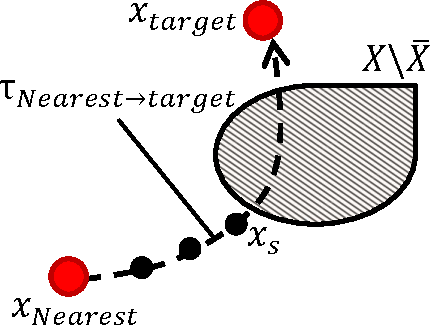
\includegraphics[width=0.2\textwidth]{Immagini/pdf/Steer_01.pdf} \label{fig:Extend_01}} \quad
\subfloat[]{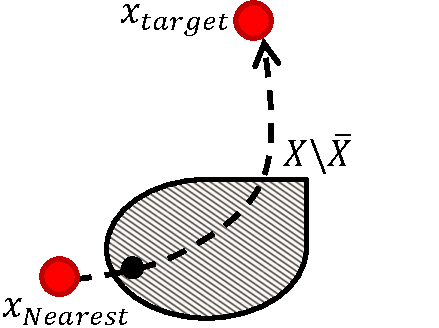
\includegraphics[width=0.2\textwidth]{Immagini/pdf/Steer_02.pdf} \label{fig:Extend_02}}
\caption{The dashed curves in both pictures are the optimal trajectories connecting the pair of states $x_{Nearest}$,$x_{target}$, while the filled areas are regions of $X$ not allowed by constraints.	
	The steering procedure integrates with a fixed step the optimal trajectory, with the aim of finding the furthest admissible state from $x_{Nearest}$ lying along the trajectory. For the example on the right, the steering is not possible: the first state obtained is returned as $x_s$ although is not valid.}
	\label{fig:Steer}
\end{figure}


% \footnote{Notice that in the general case, it is not guaranteed that $C(\tau_{ 1 \rightarrow 2}) = C(\tau_{ 2 \rightarrow 1})$}. 
The Nearest Neighbour procedure relies on the definition of a cost function $C(\tau)$. Therefore, the closeness of states does not take into account the shape of $\underline{\mathcal{X}}$.
The algorithm terminates when a steered configuration $x_s$ sufficiently close to $x_f$ is found.     
\\
\\
The previously described algorithm can be modified to consider a bidirectional strategy, expanding simultaneously two different trees \cite{RRT_bid} (see the picture in the middle of Figure \ref{fig:Tree_Comparison}). Indeed, at every iteration one of the two trees is extended toward a random state. Then, the other tree is extended toward the steered state previously obtained. At the next iteration, the roles of the trees are inverted. The algorithm stops, when the two trees meet each other. The detailed pseudocode is reported by Algorithm \ref{alg:RRT_bid}.

\begin{algorithm}
\caption{Bidirectional RRT}\label{alg:RRT_bid}
\begin{algorithmic}[1]
\Procedure{RRT bidirectional search}{$x_o$, $x_f$} 
\State $T_{master}= T(x_o)= \lbrace x_o \rbrace$;  
\State $T_{slave} = T(x_f)= \lbrace x_f \rbrace$; 
\For{\texttt{k=1:$\frac{I}{2}$}}
	\State \texttt{sample a}\,\,\, $x_R \in  \mathcal{X}$; 
	\State $x_s =$ Expand($T_{master} , x_R$) ;
	\If{\texttt{$x_s \in \underline{X}$} }
		\State $x_{s2} =$ Expand($T_{slave} , x_s$) ;
		\If{\texttt{$x_{s2} \in \underline{X}$} AND \texttt{$\Vert x_s - x_{s2} \Vert \leq \epsilon$}}
		\State $Path_1=$Path to root($x_s$);
		\State $Path_2=$Revert(Path to root($x_{s2}$));
		\State \Return $Path_1 \cup Path_2$;
		\EndIf
	\EndIf
	\State Swap($T_{master}$, $T_{slave}$);
\EndFor
\EndProcedure
\end{algorithmic}
\end{algorithm}

This solution offers several advantages. For instance, the computational times absorbed by the Nearest Neighbour search is reduced since this operation is done separately for the two trees and each tree contains at an average half of the states computed (see Section \ref{Sec:cmpt_time_serial}).
\\
\\
Notice that there are many (possibly infinite) $\tau_{o \rightarrow f} \subset \underline{ \mathcal{X} }$. Among the aforementioned set, we might be interested in finding the trajectory minimizing $C(\tau_{o \rightarrow f})$. 
The basic version of the RRT algorithm is proved to find with a probability equal to 1, a suboptimal solution \cite{RRT_star}.
The optimality issue is addressed by a variant of the RRT, called RRT* \cite{RRT_star}, whose pseudocode is contained in Algorithm \ref{alg:RRT_star} ($d$ is the cardinality of $\mathcal{X}$).
Essentially, the RRT* version, after inserting in the search tree a newer steered state, tries to undertake local improvements to the connectivity of the tree, in order to minimize the cost-to-go of the states in the $Near$ set. This is proved to converge to the optimal solution. 
There are no precise stopping criteria for the RRT*.
\\
Figure \ref{fig:Tree_Comparison} reports some examples of trees obtained by following the three exposed strategies on the use-case detailed in Section \ref{sec:probl_1}.

%\\
%Figure \ref{fig:Extend} summarizes the computation steps involved in the tree expansion, while 
%Figure \ref{fig:Tree_Comparison} reports some examples of trees obtained by following the three exposed strategies on the use-case detailed in Section \ref{sec:probl_1}.

\begin{algorithm}
\caption{RRT*}\label{alg:RRT_star}
\begin{algorithmic}[1]
\Procedure{RRT* search}{$x_o$, $x_f$} 
\State $T(x_o)=\lbrace x_o \rbrace$; 
\State $Sol=\emptyset$;
\For{\texttt{k=1:$I$}}
	\State \texttt{sample a}\,\,\, $x_R \in  \mathcal{X}$; 
	\State $x_s =$Expand star($T , x_R$);
	\If{\texttt{$x_s \in \underline{\mathcal{X}}$} AND \texttt{$\Vert x_s - x_f \Vert \leq \epsilon$}}
		\State $Sol= Sol \cup x_s$;
	\EndIf
\EndFor
\State $x_{best} = \underset{x_S \in Sol}{\operatorname{argmin}}$( Cost to root($x_S$) );
\State \Return Path to root$(x_{best}) \cup x_f$;
\EndProcedure
\\
\Procedure{Expand star}{$T,x_R$}
\State $x_s$=Expand($T,x_R$);
\State $N=size(T)$;
\State $Near=\lbrace x_i \in T | C(\tau_{i \rightarrow s}) <= \gamma {(\frac{log(N)}{N})}^{\frac{1}{d}}  \rbrace$;
\State Rewird($Near,x_s$);
\State \Return $x_s$;
\EndProcedure
\\
\Procedure{Rewird}{$Near,x_s$}
\State $x_{best fath} = x_{Nearest}$, $C_{min} = C(\tau_{Nearest \rightarrow s})$;
\For{\texttt{$x_n \in Near$}}
\If{\texttt{$\tau_{n \rightarrow s} \subset \underline{\mathcal{X}}$} AND \texttt{$C(\tau_{n \rightarrow s}) < C_{min}$}}
\State $C_{min}=C(\tau_{n \rightarrow s})$; $x_{best fath}=x_n$;
\EndIf
\EndFor
\State $Fath(x_s)=x_{best fath}$;
\State $C_s=$Cost to root($x_s$); 
\For{\texttt{$x_n \in Near$}}
\If{\texttt{$\tau_{s \rightarrow n} \subset \underline{\mathcal{X}}$}}
	\State $C_n=C(\tau_{s \rightarrow n}) + C_s$
\If{\texttt{$C_n <$ Cost to root($x_n$)}}
	\State $Fath(x_n)=x_s$;
\EndIf
\EndIf
\EndFor
\EndProcedure
\\
\Procedure{Cost to root}{$x_i$}
\State \Return $\sum_{x_p \in Path to root(x_i)} C(\tau_{Fath(p) \rightarrow p})$;
\EndProcedure
\end{algorithmic}
\end{algorithm}



%\begin{figure}
%	\centering
%\subfloat[]{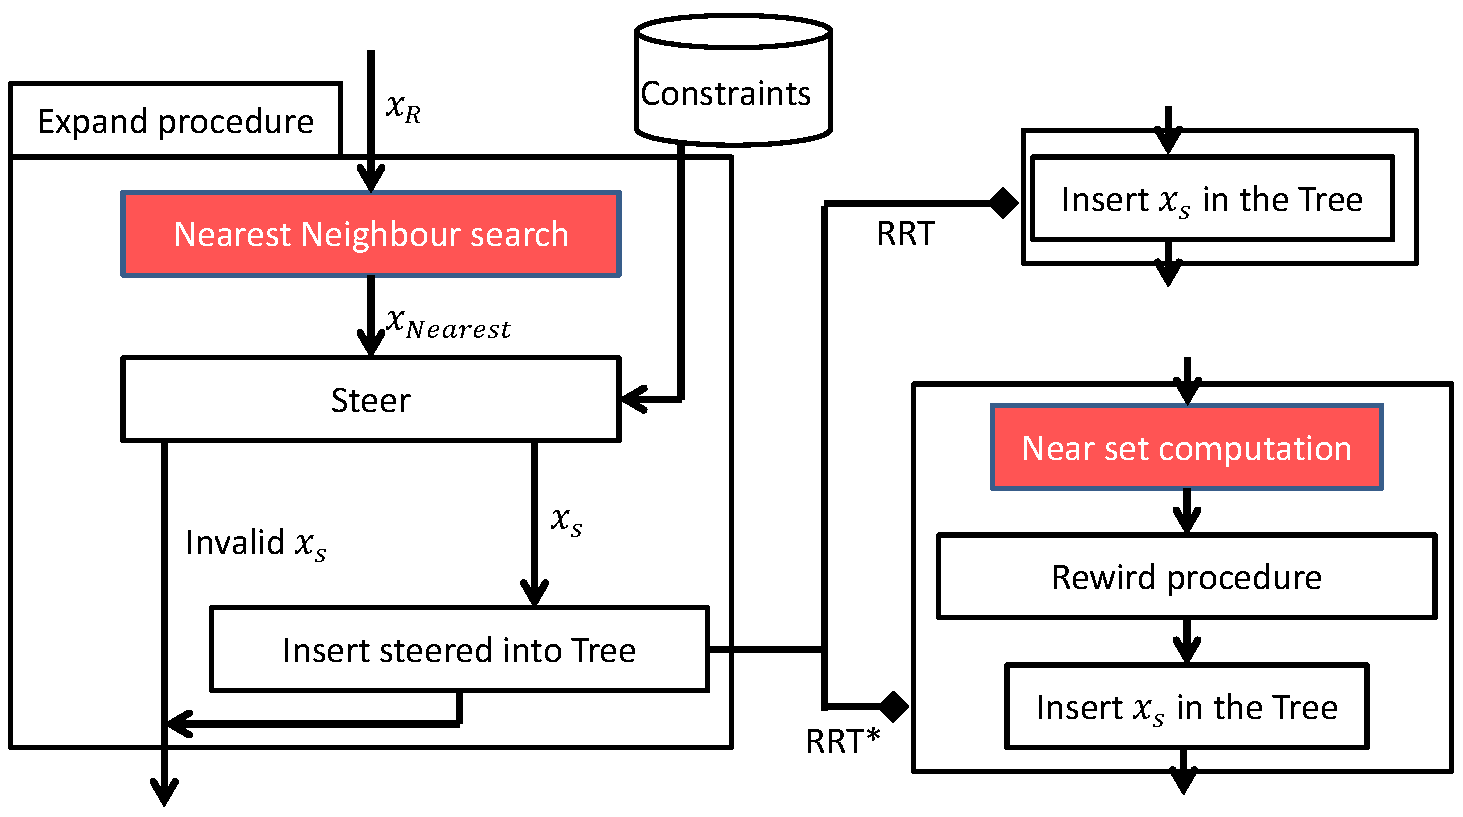
\includegraphics[width=0.5\textwidth]{Immagini/pdf/Expand.pdf} \label{fig:Extend_01}}
%\caption{Steps involved for extending the search tree(s). 
%Those operations that require to scan every element contained in the search tree are shaded with a red color.}
%	\label{fig:Extend}
%\end{figure}
   
%\begin{figure}
%	\centering
%\subfloat[]{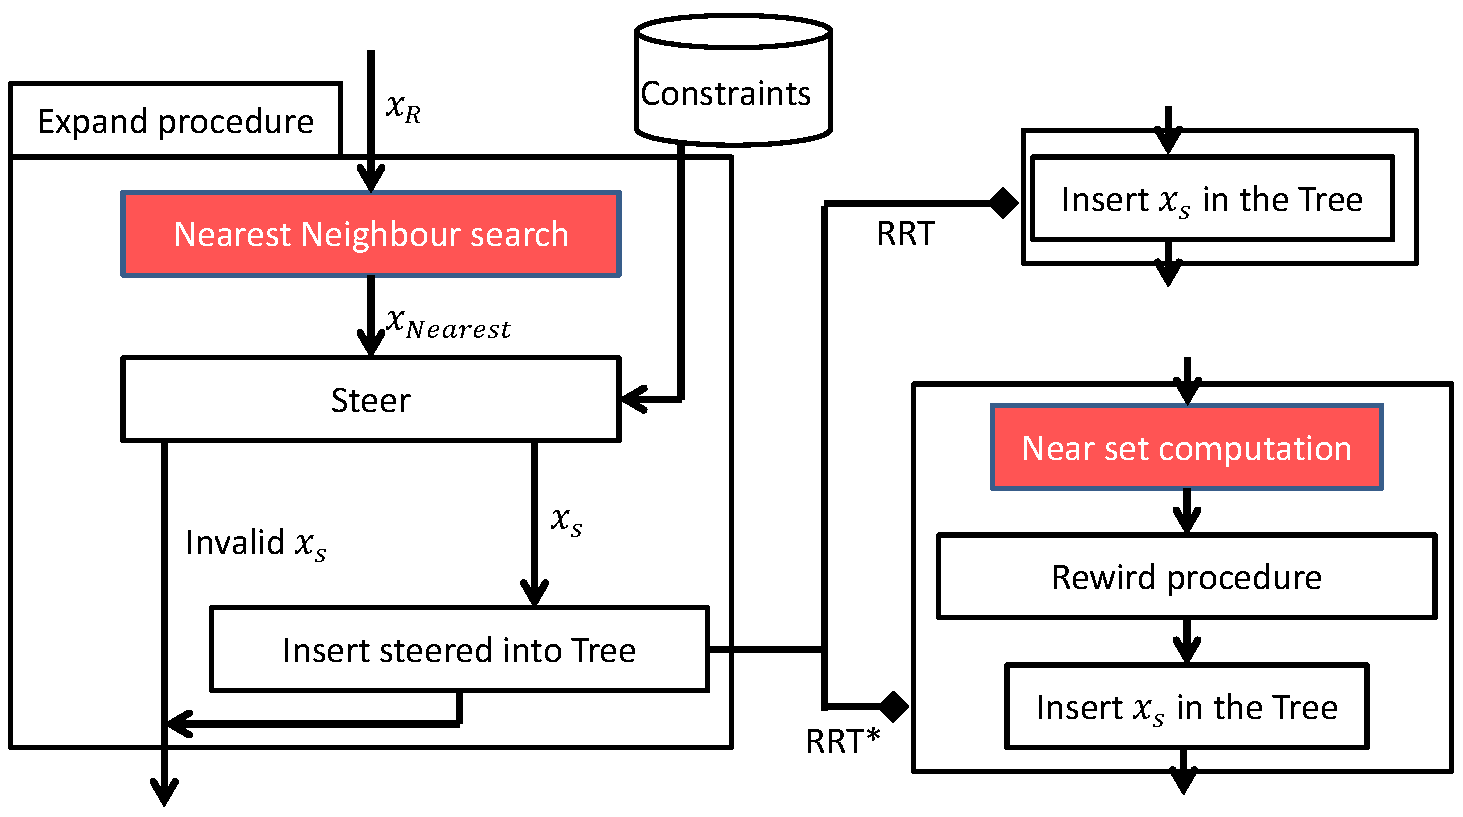
\includegraphics[width=0.5\textwidth]{Immagini/pdf/Expand.pdf} \label{fig:Extend_01}}\\
%\subfloat[]{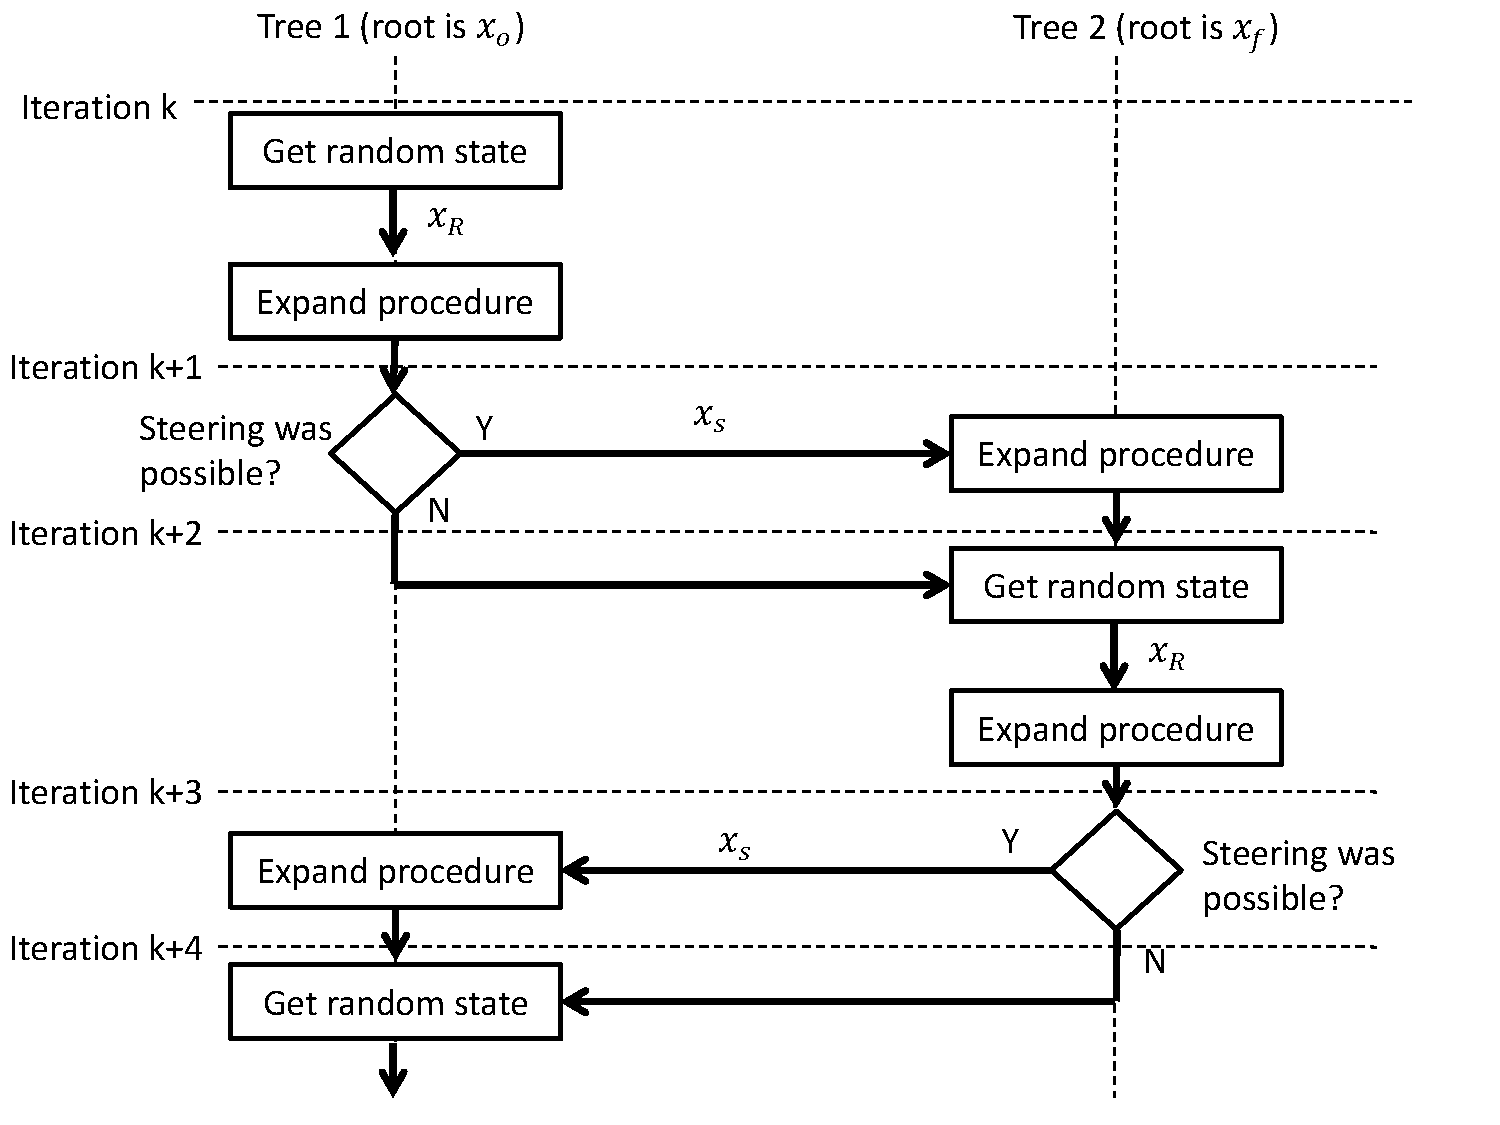
\includegraphics[width=0.5\textwidth]{Immagini/pdf/Expand_bid.pdf} \label{fig:Extend_02}}
%\caption{Steps involved for extending the search tree(s). On the top: considering the basilar version of RRT and the RRT* one; on the bottom the bidirectional formulation. 
%In the top picture, those operations that require to scan every element contained in the search tree are shaded with a red color.}
%	\label{fig:Extend}
%\end{figure}

\subsection{Computational time analysis} \label{Sec:cmpt_time_serial}

Let $t_{\tau}$ denotes the mean time absorbed by the computation of an optimal trajectory $\tau$ connecting two states and $t_{V}$ the mean time required to check whether a certain state $x$ is contained within $\underline{X}$. The proportion between the two aforementioned quantities can vary a lot, considering the specific planning problem addressed.  
The total computation time $T$ absorbed by the invocation of a basic RRT algorithm can be estimated as follows:
\begin{eqnarray}
T &=& T_{\tau} + T_V \nonumber\\
T_{\tau} & = & \mathcal{O} \left( \sum_{i=1}^I ((i+1)t_{\tau}) \right) = O \left( \frac{I(I+1)}{2} t_{\tau} \right) \nonumber\\
T_{V} & = & \mathcal{O} \left( I t_V \right) 
\label{eq:T_serial_single}
\end{eqnarray}
where $I$ is the number of iterations needed to complete the search. 
Indeed, at every iteration $i$, in the worst case, the tree contains $i$ elements for which the nearest neighbour search absorbs $i$ evaluations of $\tau$; while every expansion of the tree requires at least one feasibility check. 
\\
When considering the bidirectional version, assuming the same value for $I$, we have roughly half of the nodes in every tree and therefore the time spent for the Nearest Neighbour search changes, leading to:
\begin{eqnarray}
T_{\tau} = \mathcal{O} \left( \frac{I(I+1)}{4} t_{\tau} \right)
\label{eq:T_serial_bid}
\end{eqnarray}
Finally, when considering the RRT* formulation, the Near set determination and the evaluation of the possible reconnection (also called rewirds) drastically improves the computational time $T$, leading to:
\begin{eqnarray}
T &=& T_{\tau} + T_V \nonumber + T_{Rew}\\
T_{\tau} &= & \mathcal{O} \left(  I(I+1) t_{\tau} \right) \nonumber\\ 
T_{Rew} &= & \mathcal{O} \left( \gamma t_V \sum_{i=1}^I \left( \frac{log(i)}{i}^{\frac{1}{d}} \right)  \right)
  \label{eq:T_serial_star}
\end{eqnarray}
%assuming the same $T_V$ of equation \ref{eq:T_serial_single}.

\begin{figure}
	\centering
	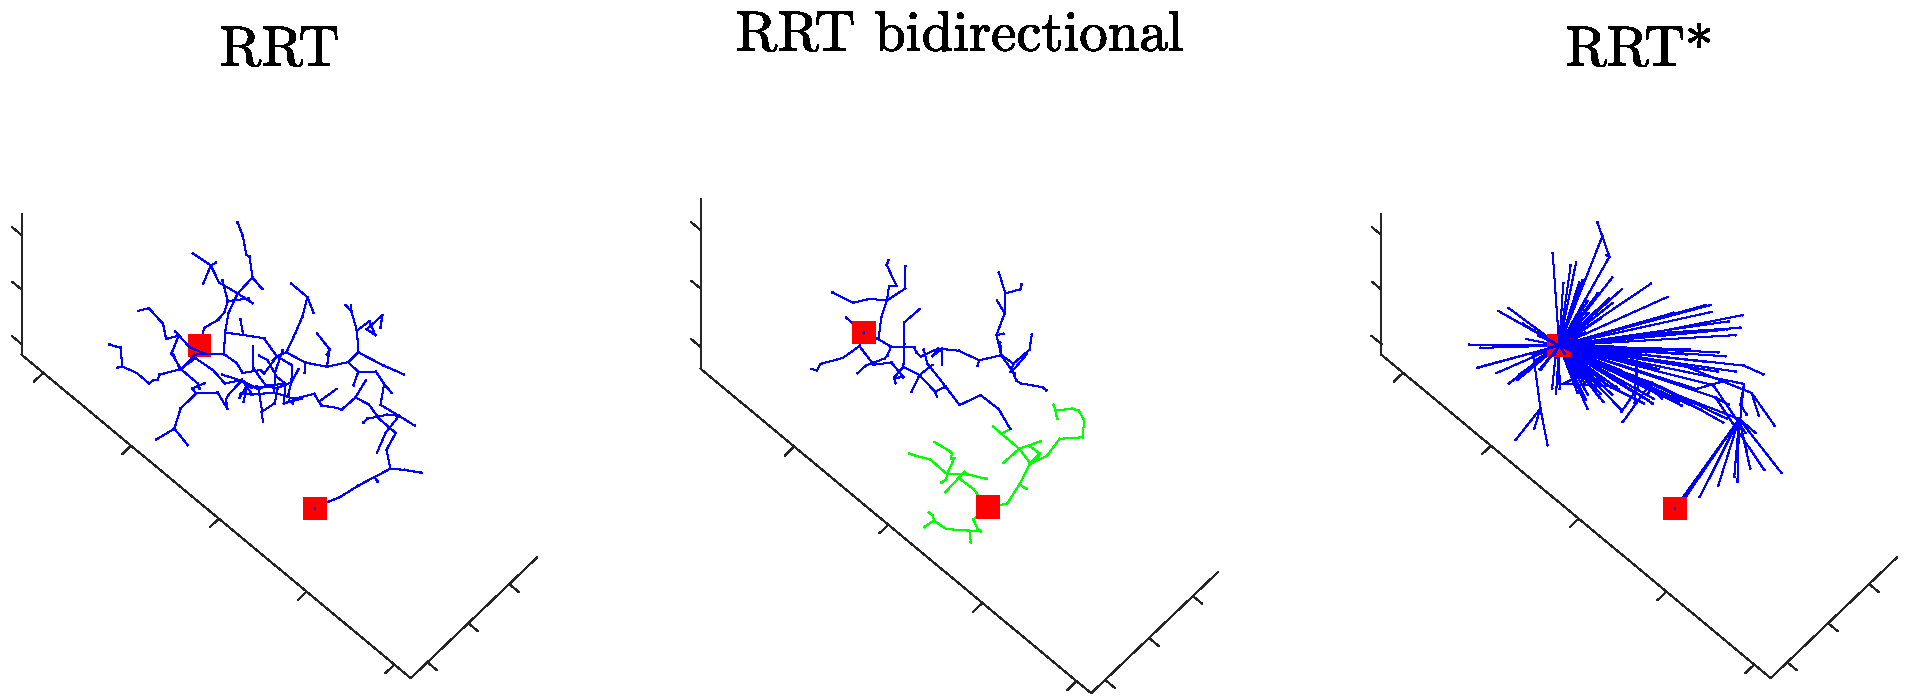
\includegraphics[width=0.5\textwidth]{Immagini/pdf/Tree_comparison_Chiara.pdf}
\caption{Examples of trees obtained when solving the planning problem detailed in Section \ref{sec:probl_1}. In all the pictures the states $x_o$ and $x_f$ are depicted as big red squares. 
%The nodes in the tree resulting by applying the RRT* have a reduced cost to go 
%( trajectories  connecting the states are simple segments in the joint space, whose cost is assumed to be the length of such a segment). 
 }
	\label{fig:Tree_Comparison}
\end{figure}

\section{MT-RRT strategies}
\label{sec:cap_03}
The aim of this Section is to show how the RRT algorithms are parallelized by making use of MT-RRT.
As already exposed, the proposed library exploits a multithreading environment, whose peculiarity is the presence of a common memory shared by threads. This characteristic requires to design accurately the critical regions, i.e. those parts of the program where threads are allowed to modify (one at a time) the values of the shared variables. 
In the following, the four possible strategies adopted by MT-RRT will be exposed.

\subsection{Parallelization of the querying activities}
\label{subsec:MT_01}

By the analysis of equations (\ref{eq:T_serial_single}), (\ref{eq:T_serial_bid}) and (\ref{eq:T_serial_star}), it is clear that the querying operations (i.e. the ones requiring to scan the entire list of elements of a tree) are computationally demanding. Therefore, the first possible strategy for a parallelization could simply consist in executing collectively (among threads) the Nearest Neighbour search and the determination of the Near set.
Clearly, it is inefficient to re-open and close a new parallel region every time a new collective search is required, but it is more convenient to launch a pool of threads at the beginning of the algorithm and then use a shared barrier to notify to threads the need to execute a newer collective search \footnote{Which is implemented as a parallel for, with a subsequent reduction operation.}. 
The maintenance operations on the search tree are executed always by the main thread.
The mean computation time expected when considering a perfect parallelization and adopting $P$ threads can be estimated as follows:
\begin{eqnarray}
T(P) &=& \frac{T_{\tau}}{P} + T_V \nonumber\\
\textit{for RRT*  \,\,\,\,\,} T(P) &=& \frac{T_{\tau}}{P} + T_V + T_{Rew} 
\end{eqnarray}
%Therefore, this strategy is expected to be beneficial only for those cases for which $t_{\tau}$ is much more greater than $t_V$.
  
\subsection{Parallel exploration on a shared tree}
\label{subsec:MT_02}

Another way to obtain a parallelization is to actually do simultaneously, every single step of the algorithms detailed in Section \ref{sec:cap_02}. Therefore, we can imagine having threads sharing a common tree, executing in parallel every step of the expansion process. Some critical regions must be designed to allow the threads executing the maintenance of the shared tree (inserting new nodes or executing new rewirds) one at a time.
Ideally, the computation time of this solution can be estimated as follows:
\begin{eqnarray}
T(P) &=& \frac{T_{\tau} + T_V }{P} \nonumber\\
\textit{for RRT*  \,\,\,\,\,} T(P) &=& \frac{T_{\tau} + T_V + T_{Rew} }{P}
\label{eq:T_parall_02}
\end{eqnarray}
However, the presence of the critical regions can severely compromise the efficiency of the parallelization for certain planning problem, enlarging the total overhead times. Indeed, the computational times obtained by adopting this strategy could be far beyond the time described by equation (\ref{eq:T_parall_02}) (see Section \ref{sec:cap_04}).

\subsection{Parallel expansions of copied trees}
\label{subsec:MT_03}

To limit as much as possible the overheads induced by the presence of critical regions, we can consider a version similar to the one proposed in the previous Section, in which every thread has a private copy of the search tree. After a new node is added by a thread to its own tree, $P-1$ copies are computed and dispatched to the other threads. At every iteration, all the threads take into account the list of nodes received from the others and insert some of them into their private trees. This mechanism is able to avoid the
simultaneous modification of a tree by two different threads, avoiding the use of critical regions. 
The pseudocode of this solution is reported in Algorithm \ref{alg:RRT_single_MT_02}.

\begin{algorithm}
\caption{}\label{alg:RRT_single_MT_02}
\begin{algorithmic}[1]
\Procedure{Tree copies search}{$x_o$, $x_f$, $P$}
\State $Path = \emptyset$;
\For{\texttt{kp=1:$P$}} 
\State $T_{kp}=\lbrace x_o \rbrace$;
\State $J^{kp}=\emptyset$;
\State $C_{kp}=0$;
\State \texttt{launch thread}( Thread search($kp$));
\EndFor
\State \Return $Path$;
\EndProcedure
\\
\Procedure{Thread search}{$th_{id}$}
\For{\texttt{k=1:$\frac{I}{P}$}}
	\If{$Path \neq \emptyset$} 
	\Return;
	\EndIf
	\State $S=size(J^{th_{id}})$;
	\For{\texttt{kj=1:($S-C_{th_{id}}$)}}
		\State $C_{th_{id}}=C_{th_{id}}+1$;
		\State $T_{th_{id}} = T_{th_{id}} \cup J^{th_{id}}_{kj}$;
	\EndFor
	\State \texttt{sample a}\,\,\, $x_R \in  \mathcal{X}$;
	\State $x_s =$ Expand($T_{th_{id}} , x_R$) ;
	\If{\texttt{$x_s \in \underline{\mathcal{X}}$ } AND \texttt{$\Vert x_s - x_f \Vert \leq Threshold$}}
		\State \texttt{critical region begin}
		\State $Path=$ Path to root$(x_s) \cup x_f$;	
		\State \texttt{critical region end}
			\For{\texttt{kp=1:$P$}}
			\If{\texttt{kp != $th_{id}$}}
			\State $j_{kp}=x_s$; \Comment copy this node
			\State $J_{kp}= J_{kp} \cup j_{kp}$;
			\EndIf
			\EndFor
		\State \Return;
	\EndIf
\EndFor
\EndProcedure
\end{algorithmic}
\end{algorithm}

When considering the bidirectional strategy, the mechanism is analogous but introducing for every thread  a private copy of both the searching trees. Instead, for the RRT* formulation, every thread communicates to the others not just the new states found, but also the rewirds executed.
Moreover, a common list of solutions found is maintained during the expansions. At the end of all the explorations, the path in that list minimizing the cost $C(\tau)$ is returned.
In this way, when following this approach, there is no need to synchronize threads for executing rewirds.
Assuming to $t_M$ equal the time required to copy a node inserted in the tree, the expected computation time of this strategy turns out to be:
\begin{eqnarray}
T(P) &=& \frac{T_{\tau} + T_V }{P} + T_M  \nonumber\\
\textit{for RRT*  \,\,\,\,\,}  T(P) &=& \frac{T_{\tau} + T_V + T_{Rew} }{P} + T_M \nonumber\\
T_M  & = & \mathcal{O} \left(  \frac{I(P-1)}{P} t_M \right)
\end{eqnarray}  

\subsection{Blinded multiagents explorations}
\label{subsec:MT_04}

The strategy proposed in this Section aims at exploiting a significant number of threads, with both a  reduced synchronizing need and allocation memory requirements.
To this purpose, we have developed a variant of the RRT for which every exploring thread has not the entire knowledge of the tree, but it is conscious of a small portion of it. Therefore, we can deploy many threads to simultaneously explore the region $\underline{X}$ (ignoring the results found by the other agents) for a certain amount of iterations $N_b$. After completing this sub-exploration, all data incoming from the agents are collected and stored in a centralized data base while the agents wait to begin a new explorative batch, completely forgetting the nodes found at the previous iteration. 
The described behaviour resembles one of many exploring ants, which reports the exploring data to a unique anthill.  The pseudocode in Algorithm \ref{alg:RRT_agents} details the proposed approach. The total amount of iterations $I$ is split into $C$ cycles of $N_b$ explorations for every agent(thread). 
Clearly $I \simeq N_b (P-1) C$.

\begin{algorithm}
\caption{Multi Agent RRT}\label{alg:RRT_agents}
\begin{algorithmic}[1]
\Procedure{Background}{$x_o$, $x_f$, $P$}
\State $T_M=\lbrace x_o \rbrace$; 
\For{\texttt{kp=1:$P$}}
\State $T_{kp} = \emptyset$;
\State \texttt{launch thread}(Agent work($kp$));
\EndFor
\State $k=0$;
\While{$k < I$}
	\For{\texttt{kp=1:$P$}}
	\State \texttt{sample a} $x_R \in T_M \vert \mathbb{P}(x_i) \propto \frac{1}{1+C(\tau_{i \rightarrow f})}$;
	\State $T_{kp} = \lbrace x_{R} \rbrace$;
	\EndFor
	\State \texttt{threads barrier};
	\State \texttt{threads barrier};
	\State $T_M = \lbrace T \cup T_1, \cdots, T_P \rbrace$;
	\If{\texttt{$\exists x_i \in T_M s.t. \Vert x_i - x_f \Vert \leq \epsilon$}}
		\State \texttt{Kill agents};
		\State \Return Path to root($x_i$)$ \cup x_f$;	
	\EndIf
	\State $k=k+N_b \cdot P$;
\EndWhile
	\State \texttt{Kill agents};
\EndProcedure
\\
\Procedure{Agent work}{$th_{id}$}
\While{\texttt{TRUE}}
	\State \texttt{threads barrier};
	\If{$T_{th_{id}} = \emptyset$}
	\State \texttt{break};
	\EndIf
\State RRT search(); \Comment{on $T_{th_{id}}$, with $I=N_b$};
	\State \texttt{threads barrier};
\EndWhile
\EndProcedure
\\
\Procedure{Kill agents}{}
	\For{\texttt{kp=1:$P$}}
	\State $T_{kp} = \emptyset$;
	\EndFor
	\State \texttt{threads barrier};
\EndProcedure
\end{algorithmic}
\end{algorithm}

Notice that there is no need to physically copy the states computed by the agents when inserting them into $T_M$, since threads share a common memory: a reference to the newer states is simply added to $T_M$. When considering this approach a bidirectional search is not implementable, while the RRT* can be extended as reported in Algorithm \ref{alg:RRT_agents_star}.


\begin{algorithm}
\caption{Multi Agent RRT*}\label{alg:RRT_agents_star}
\begin{algorithmic}[1]
\Procedure{Multi Agent search *}{$x_o$, $x_f$, $P$}
\State $T_M={x_o}$; 
\For{\texttt{kp=1:$P$}}
\State $T_{kp} = \emptyset$;
\State \texttt{launch thread}(Agent work * ($kp$) );
\EndFor
\State $Sol = \emptyset$;
\State $k=0$;
\While{$k < I$}
	\For{\texttt{kp=1:$P$}}
	\State \texttt{sample a} $x_R \in T_M \vert \mathbb{P}(x_i) \propto \frac{1}{1+C(\tau_{i \rightarrow f})}$;
	\State $T_{kp} = \lbrace x_{kp} \rbrace$;
	\State $Near^{kp}=\lbrace x_i \in T_M | C(\tau_{i \rightarrow s}) <= \gamma {(\frac{log(N)}{N})}^{\frac{1}{d}}  \rbrace$;
	\State $T_{kp}=\lbrace T_{kp} \cup$ Path to root($x^{kp}$) $ \,\,\,\, \forall x^{kp} \in Near^{kp} \rbrace$
	\EndFor
	\State \texttt{threads barrier};
	\State \texttt{threads barrier};
	\State $T_M = \lbrace T \cup T_1, \cdots, T_P \rbrace$;
	\For{$x_m \in \lbrace x | x \in T_p \bigwedge \Vert x - x_f \Vert \leq \epsilon \,\,\, \forall p=1, \cdots, P \rbrace$}
		\State $Sol = Sol \cup x_m$;	
	\EndFor
	\State $k=k+N_b \cdot P$;
\EndWhile
	\State \texttt{Kill agents};
	\State $x_{best} = \underset{x_S \in Sol}{\operatorname{argmin}}$( Cost to root$(x_S)$ );
	\State \Return Path to root$(x_{best}) \cup x_f$;
\EndProcedure
\\
\Procedure{Agent work *($th_{id}$)}{}
\While{\texttt{TRUE}}
	\State \texttt{threads barrier};
	\If{$T_{kp} = {\emptyset}$}
	\State \texttt{break};
	\EndIf
\State RRT* search(); \Comment{on $T_{kp}$, with $I=N_b$};
	\State \texttt{threads barrier};
\EndWhile
\EndProcedure
\end{algorithmic}
\end{algorithm}

When considering this formulation, we are modifying the canonical behaviour of an RRT algorithm, since agents explore every time some new roots, ignoring all the previously computed nodes. However, we empirically found that the global behaviour of the path search is not deteriorated. In particular, the optimality properties of the RRT* seems to be preserved, see Figure \ref{fig:Problem_A_04}.

The mean computation time of this kind of strategy can be estimated as follows:
\begin{eqnarray}
T(P) &=& \frac{T_{\tau} + T_V}{P} \nonumber\\
\textit{for RRT* \,\,\,\,\,}   
T(P) &=& \frac{T_{\tau} + T_V + T_{Rew}}{P}   \nonumber\\
T_{\tau} & = & \mathcal{O} \left( C (N_b+1)N_b t_{\tau} \right) \nonumber\\
T_{Rew}  & = & \mathcal{O} \left( C \gamma t_V \sum_{i=1}^{N_b} \left( \frac{log(i)}{i}^{\frac{1}{d}} \right) \right)  
\end{eqnarray}
 
The mean time spent for the querying operations is considerably lower, since such operations are performed by agents considering only their own local reduced size trees. 

%\section{Multiprocess strategies}
%Multiprocess (MP) programs aim at exploiting a set of concurrent processes to get in a faster way a solution to a complex problem. Every process has its own private variables and some unified protocol (METTERE ref a MPI o ad altri interprocess comm) can be exploited to let processed exchange informations, synchronizing their efforts.
For this reason the strategies METTERE le prime due MT are very difficult to be translated in MP environments; while the strategy METTERE can be in principle extended to MP, considering to exploit the communication between processes to notify the results found by a process to the others.
However, this approach would absorb much more computation time than a multithreading one, when considering the same number of threads/processes, since the communication time between processes is much higher than the same for threads (since threads are able to create variables and then directly add them to a container possessed by another thread).
\\
Therefore such an approach will not be followed in this work.        

\subsection{A master-slave strategy}

The MP strategy we propose, aims at exploiting a big number of concurrent processes \footnote{Since launching a big number of concurrent processes is preferable than launching the same number of concurrent threads}, with a reduced synchronizing necessity.
To this purpose it is possible to exploit a master-slaves scheme: the master process is the only one having the entire knowledge of the search tree, while many other slave processes receive every time new roots to expand, ignoring the states computed by the other slaves.
Results from slaves are collected by the master.
The behaviour of the slaves resembles the one of many exploring ants, which reports data about the exploration to a unique centralized database (the Anthill experience).  The pseuocode in Algorithm \ref{alg:RRT_master_slave} describes this approach (the Procedure RRT search in Slave work is the same of METTERE ). The total amount of iterations $I$, is split into $C$ duty cycles. For every cycle the slaves expand the received newer roots for a maximum of $N_b$ iterations.
Clearly $I=N_b (P-1) C$ 

\begin{algorithm}
\caption{master-slaves RRT}\label{alg:RRT_master_slave}
\begin{algorithmic}[1]
\Procedure{Master work}{$P$}
\State $T(x_o)={x_o}$; 
\For{\texttt{kp=1:$P-1$}}
\State \texttt{launch} $process_{kp}$ (Slave work);
\EndFor
\State $k=0$;
\While{$k < I$}
	\For{\texttt{kp=1:$P-1$}}
	\State Sample one $x_{kp}$ from $T$);
	\State Send $x_{kp}$ to slave $kp$;
	\EndFor
	\State Wait results from slaves;
	\For{\texttt{kp=1:$P-1$}}
	\State \Comment{process results from slave $kp$};
	\State $S_{kp} = {x^{kp}_{1}, \cdots ,x^{kp}_{S}}$; 
	\For{\texttt{$x^{kp}_{s} \in S_{kp}$}}
		\State $x_{new} = x^{kp}_{s}$;
		\State $Fath(x_{new}) = Fath(x^{kp}_{s})$;
		\State Insert($T$, $x_{new}$);
		\If{\texttt{$\Vert x_{new} - x_f \Vert \leq \epsilon$}}
		\State $Path=$ Path to root$(x_{new}) \cup x_f$;
		\State Kill all slaves();
		\State \Return;
		\EndIf
	\EndFor
	\EndFor
	\State $k=k+N_b(P-1)$;
\EndWhile
\EndProcedure
\\
\Procedure{Slave work}{}
\While{\texttt{TRUE}}
\State Wait a newer root $x_{new\,root}$ to expand from Master();
\State $T=x_{new\,root}$;
\State RRT search(); \Comment{with $I=N_b$};
\State Send all nodes in $T$ to Master;
\EndWhile
\EndProcedure
\end{algorithmic}
\end{algorithm}

Notice that the computed newer states must be copied from every slave to the master (through an interprocess communication stream), but not from a certain slave to the other ones. This drastically reduce the traffic over the net of processes. 
When considering this approach a bidirectional search is not implementable, while the RRT* can be extended as reported in Algorithm METTERE.

\begin{algorithm}
\caption{master-slaves RRT*}\label{alg:RRT_star_master_slave}
\begin{algorithmic}[1]
\Procedure{Master work}{$P$}
\State $T(x_o)={x_o}$; 
\For{\texttt{kp=1:$P-1$}}
\State \texttt{launch $process_{kp}$ executing \textbf{Slave work}};
\EndFor
\State $k=0$;
\State $Sol = \emptyset$;
\State $k=0$;
\While{$k < I$}
	\For{\texttt{kp=1:$P-1$}}
	\State Sample one $x_{kp}$ from $T$);
	\State Send $x_{kp}$ to slave $kp$;
	\EndFor
	\State Wait results from slaves;
	\For{\texttt{kp=1:$P-1$}}
	\State \Comment{process results from slave $kp$};
	\State $S_{kp} = {x^{kp}_{1}, \cdots ,x^{kp}_{S}}$; 
	\For{\texttt{$x^{kp}_{s} \in S_{kp}$}}
		\State $x_{new} = x^{kp}_{s}$;
		\State Insert star($T$, $x_new$);
		\If{\texttt{$\Vert x_{new} - x_f \Vert \leq \epsilon$}}
		\State $Sol = Sol \cup x_{new}$;
		\EndIf
	\EndFor
	\EndFor
	\State $k=k+N_b(P-1)$;
\EndWhile
\State $x_{best} = argmin_{x_S \in Sol} ($ Cost to root$(x_S) ) $;
\State \Return Path to root$(x_{best}) \cup x_f$;
\EndProcedure
\end{algorithmic}
\end{algorithm}

Essentially, the rewirds are never executed by slaves (which don't have the complete knowledge of the tree), but is the master that compute the rewirds step, at the time of collecting data from slaves. For improving the efficiency, the list of results coming from the slaves can be checked for rewirds in a parallel way, exploiting threads, therefore combining multiprocess with multithreading (the results reported in Section METTERE, was obtained applied this method).


Clearly, when considering this formulation, we are modifying the behaviour of an RRT algorithm, since slaves explore new roots, ignoring all the other nodes. However, we empirically found that the global behaviour of the path search is similar to the canonical one. In particular, the properties of the RRT* are preserved, see Figure METTERE.

METTERE esempio di albero trovato con colori diversi per slave diversi e mostrare come costo della soluzione RRT* master-slave sia lo stesso di quella RRT* seriale normale, sullo use-case del robot 
a 3 gdl.

Regarding the computational issue, the mean computation time of this kind of strategy can be estimated as follows ($P_{T}$ is the number of threads adopted to parallelize the rewird operations on the list of nodes collected from slaves):
\begin{eqnarray}
\textit{ RRT  \,\,} T &\propto & \frac{(N_b+1)N_b}{2(P-1)} t_{\tau} 
+ \frac{I}{P-1} t_V + \frac{I}{P-1} t_M
\nonumber\\
\textit{ RRT*  \,\,} T &\propto & \frac{(N_b+1)N_b}{2}(\frac{1}{P-1} + \frac{1}{P_T}) t_{\tau} 
+ (\frac{I}{P-1} + \cdots \nonumber\\
&+& \frac{\gamma log(I)^{\frac{1}{d}}}{I\,P_{T}}) t_V + \frac{I}{P-1} t_M
\end{eqnarray}

The quantity $t_M$ takes into account also the time spent for communicating the results from the slaves to the master and therefore is higher than the same for the method proposed in Section METTERE. However, the mean time spent for the Nearest Neighbour search is considerably lower, since this operation is performed by the slaves processes, which reason only about its own local trees. 


\section{Performance analysis}
\label{sec:cap_04}

This Section will present the performance obtained when applying the strategies proposed in Section \ref{sec:cap_03}. The following will describe four different representative planning benchmarks, which will be employed later to show the computational times obtained applying the strategies proposed, when varying the number of threads.

\subsection{Problem 1 : path planning}
\label{sec:probl_1}

Here we consider a classical path planning problem. The robot adopted is a 3 d.o.f. robot with simplified shaped links. Every state $x \in X$ is simply the pose of the robot, i.e. the 3 values describing the angular joint displacements. The admissible region $\underline{X}$ is represented by the free configurational  space, i.e. the set of poses $x$ for which the robot is not in collision w.r.t. all the fixed obstacles populating the scene. The workspace of the robot is represented in Figure \ref{fig:Problem_1}.
An optimal trajectory $\tau_{1 \rightarrow 2}$ is the segment in the joint space whose extremals are $x_{1,2}$, and the length of such segment is considered as $C(\tau_{1 \rightarrow 2})$.
The states $x^k_s$ are obtained  by following the segment connecting $x_{Nearest}$ to $x_{target}$ with a fixed length step $l$ (apriori decided):
\begin{eqnarray}
L &=& l \cdot \frac{x_{target}-x_{Nearest}}{\Vert x_{target}-x_{Nearest} \Vert} \nonumber\\
x^k_s &=& x_{Nearest} + k \cdot L
\end{eqnarray}

\begin{figure}
	\centering
\subfloat[]{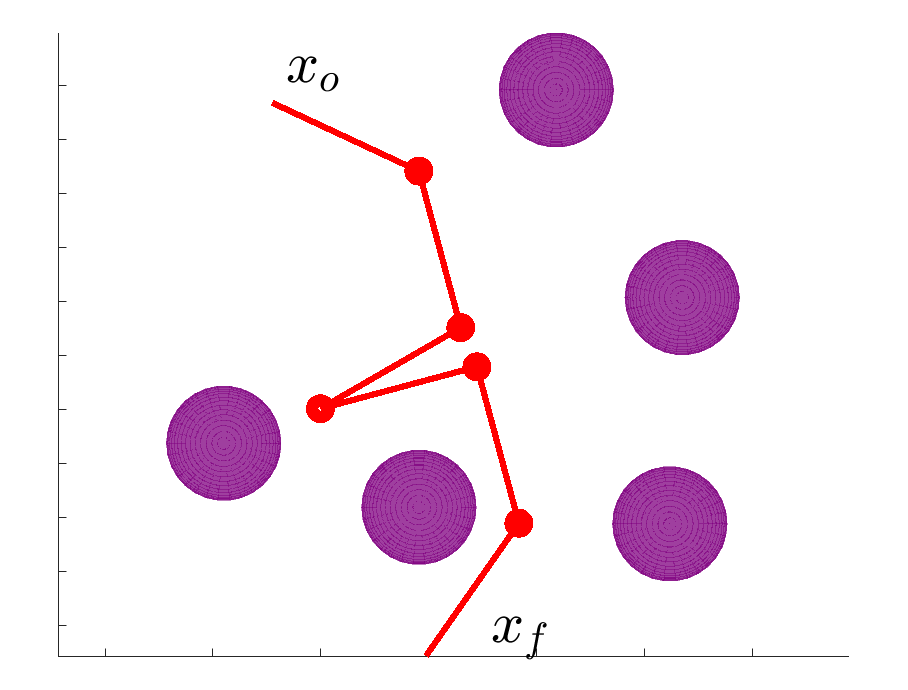
\includegraphics[width=0.2\textwidth]{Immagini/pdf/Problem_A_01.eps} \label{fig:Problem_A_01}} \quad
\subfloat[]{\includegraphics[width=0.2\textwidth]{Immagini/pdf/Problem_A_02.eps} \label{fig:Problem_A_02}} \\
\subfloat[]{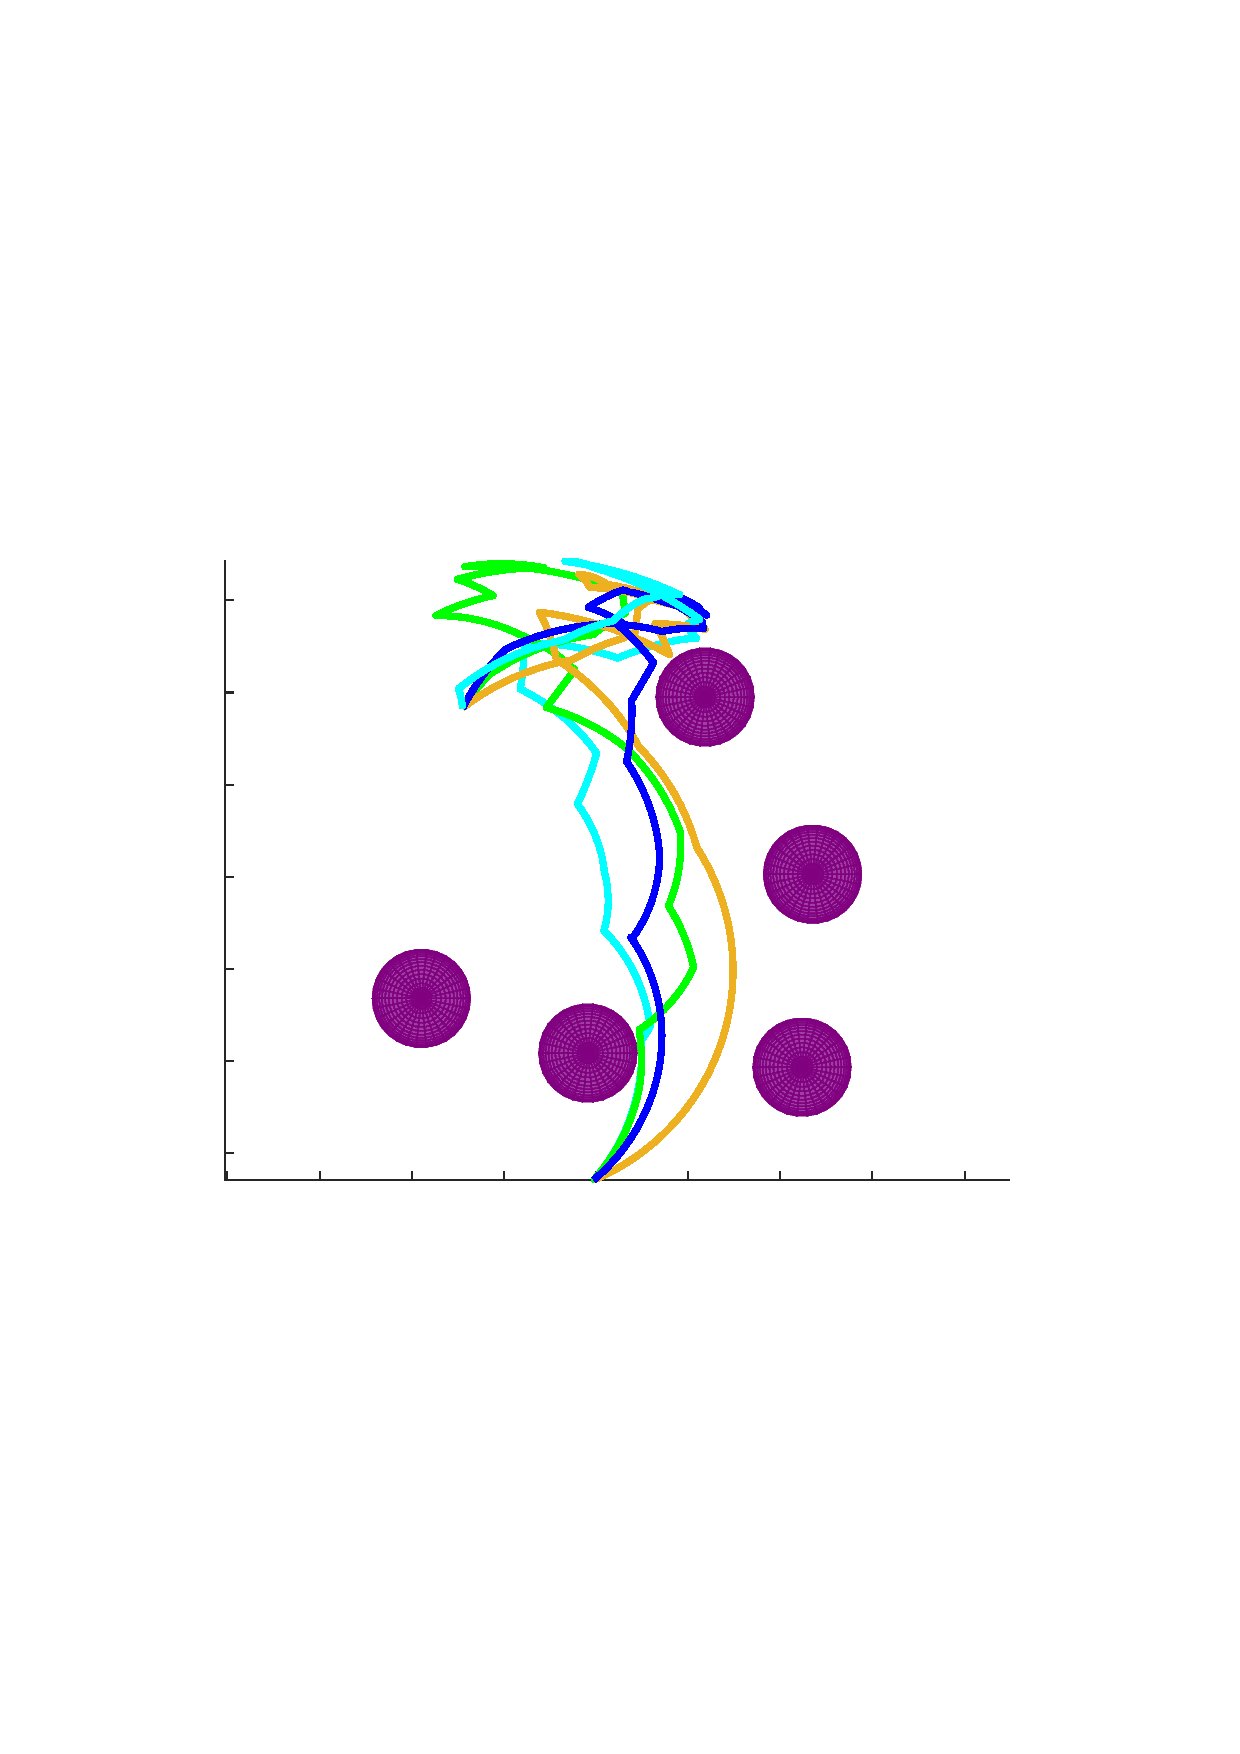
\includegraphics[width=0.2\textwidth]{Immagini/pdf/Problem_A_03.pdf} \label{fig:Problem_A_03}} \quad
\subfloat[]{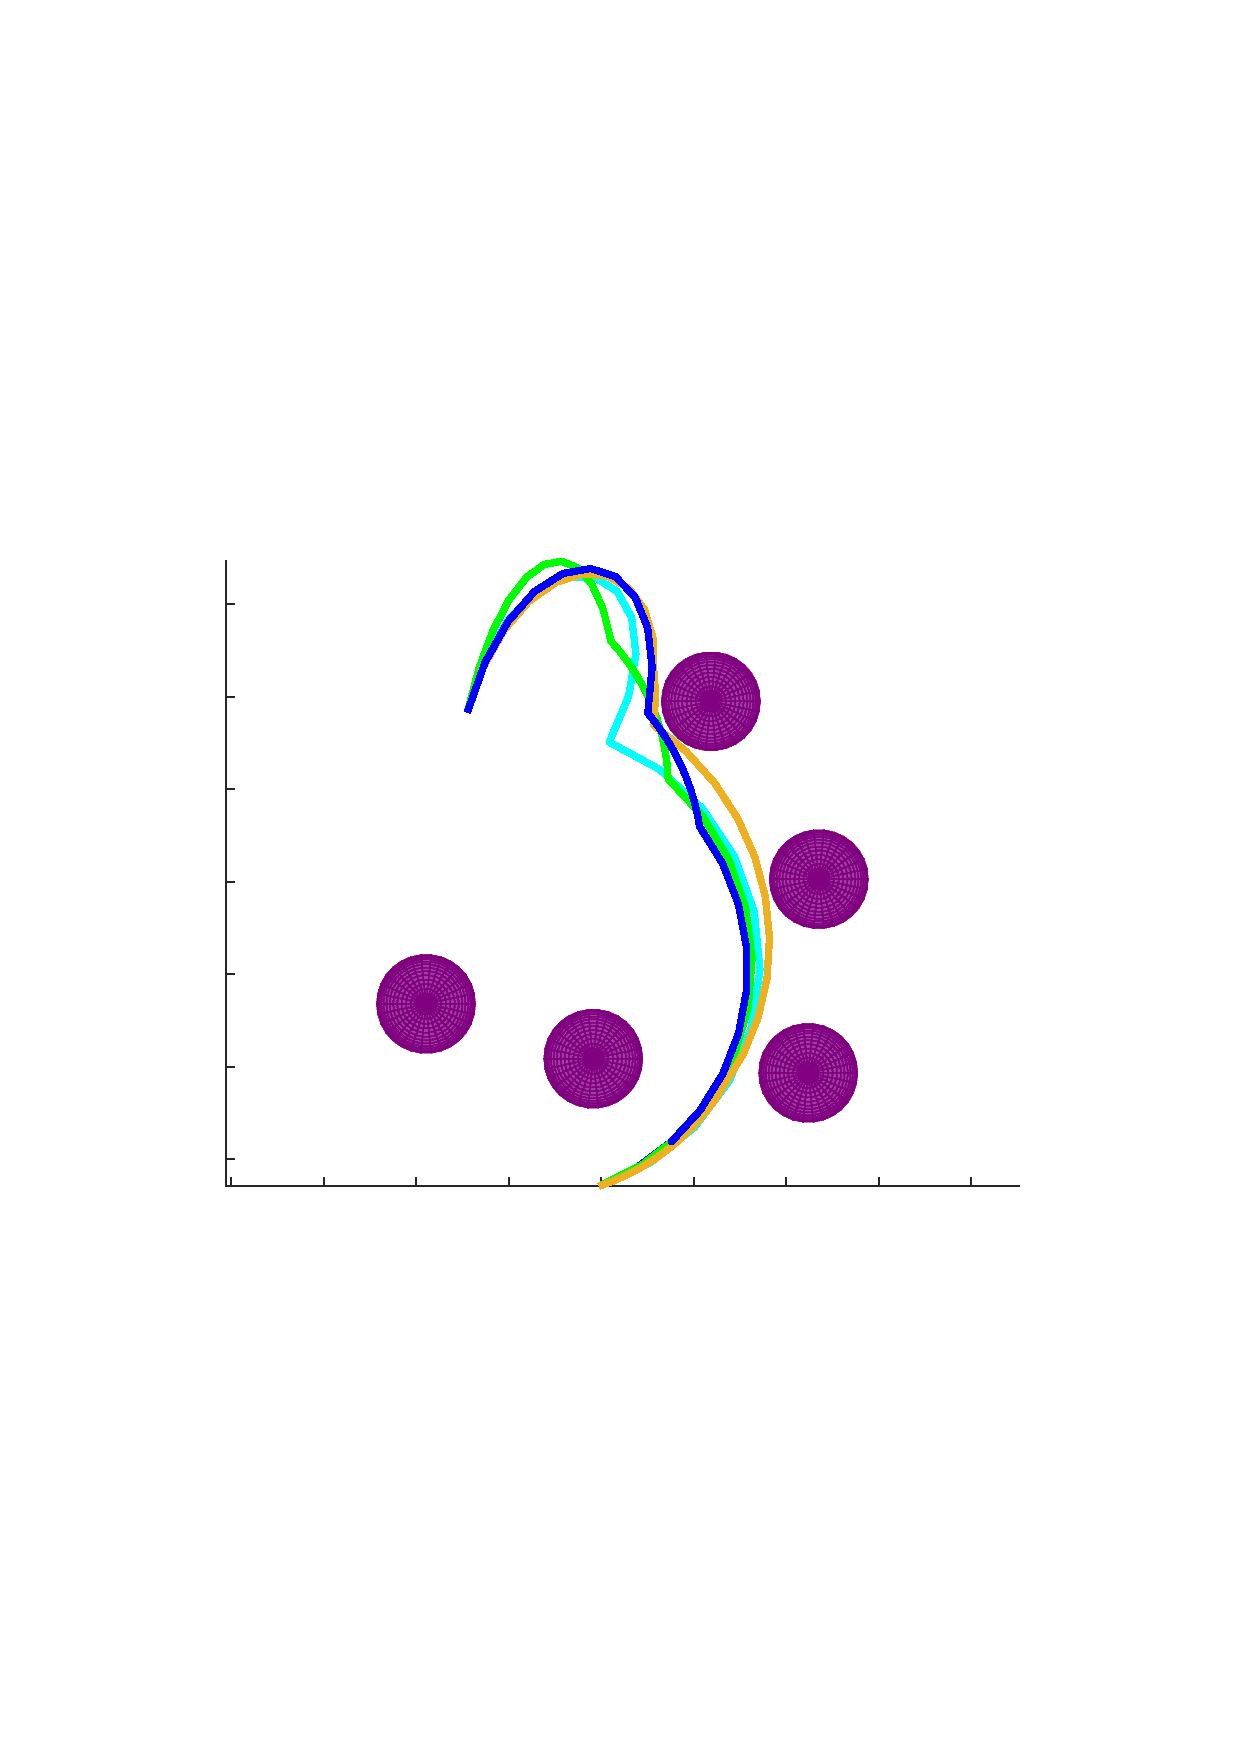
\includegraphics[width=0.2\textwidth]{Immagini/pdf/Problem_A_04.pdf} \label{fig:Problem_A_04}}
\caption{The two pictures on the top depict the planning problem considered for Problem 1. The purple spheres are the obstacles populating the workspace of the robot. On the left the poses $x_o$ and $x_f$, while on the right the optimal path obtained by applying RRT* with some intermediate poses and the trajectory of the E.E. 
The pictures at the bottom are examples of paths found when applying a standard (serial) RRT on the left; the multiagents version of RRT* described in Section \ref{subsec:MT_04} on the right.}
	\label{fig:Problem_1}
\end{figure}

\subsection{Problem 2 : path planning with a 7 d.o.f robot }
\label{sec:probl_2}

Another path planning problem is considered here, similar to the previous one and with the same workspace. 
However, here the robot considered, reported in Figure \ref{fig:Problem_2}, has 7 d.o.f. 
Notice that time $T_V$ is more than doubled with respect to Problem 1; while time $T_{\tau}$ is almost the same.    

\begin{figure}
	\centering
	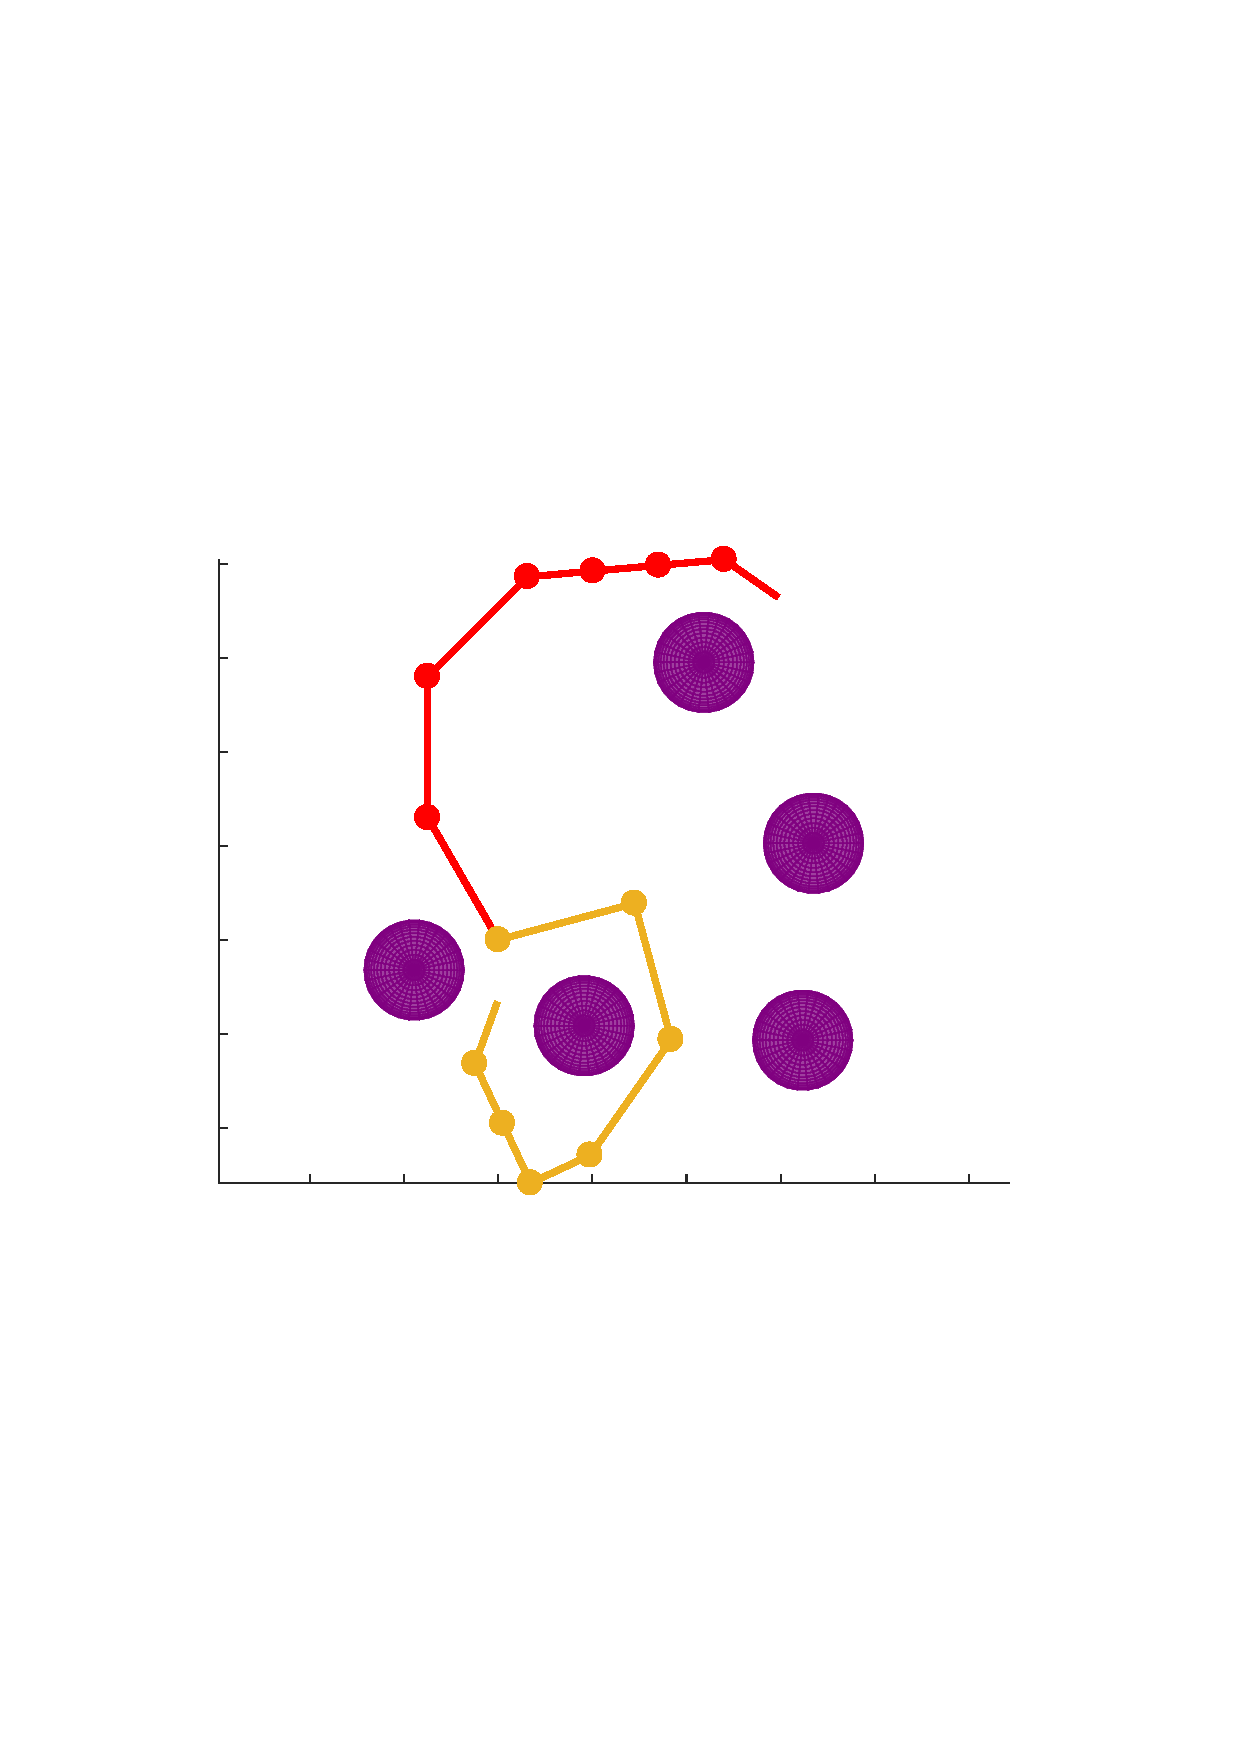
\includegraphics[width=0.2\textwidth]{Immagini/pdf/problem_7gdl.pdf} \label{fig:Problem_A_01}
\caption{The planning problem considered for Problem 2. The starting and ending poses of the robot are depicted respectively in red and in orange. }
	\label{fig:Problem_2}
\end{figure}

\subsection{Problem 3 : trajectory planning}
\label{sec:probl_3}

In this case, we consider the same scenario of Problem 1, but considering a trajectory planning problem.
The state $x$ is composed as follows:
\begin{eqnarray}
x=[ q^{T} \,\,\,\, \dot{q}^{T} ]^{T}
\end{eqnarray}
where $q$ is the pose of the robot (angular displacements), while $\dot{q}$ are the joint velocities. The second order minimum time trajectory connecting two states $x_{1,2}$ is considered as $\tau_{1 \rightarrow 2}$. Such a trajectory can be computed by making use of the Reflexxes library \cite{Reflexxes}, which takes into account the kinematic limitations of a manipulator, but not the obstacles populating the scene. The cost $C(\tau_{1,2})$ is assumed  as the time for reaching $x_2$ when following $\tau_{1,2}$. The states $x^{1,\cdots,K}_s$ considered by the steering function are separated by a (small) fixed time $\Delta t$: $x^{k}_s = \tau(k \Delta t)$.
Notice that for this case time $T_V$ is equal to the same when considering Problem 1, while time $T_{\tau}$ is significantly higher.

\subsection{Problem 4 : kinodynamic planning}
\label{sec:probl_4}

This benchmark considers an optimal control problem. Consider the following non linear dynamical system whose equation of motion is as follows:
\begin{eqnarray}
\dot{x} &=& f(x) + u \label{eq:motion_problem_4} \\  
f(x) &=& T^{-1} \cdot 
diag(-1-e^{- \alpha_{1} x_1^2}, \cdots, -1-e^{- \alpha_{6} x_6^2})
\cdot T \nonumber\\
\end{eqnarray}
where all coefficients $\alpha_{1,2,3,4,5,6}$ are $>0$, while $T$ is an orthogonal matrix.
The state-space considered for planning is clearly the state-space of the above dynamical system.
A trajectory $\tau_{1 \rightarrow 2}$ is obtained integrating eq. (\ref{eq:motion_problem_4}) forward in time, under the effect of the optimal linear regulator obtained considering a linearization of the system:
\begin{eqnarray}
\dot{x} &=& \left( f(x_1) -A x_1 \right) + A x + u \texttt{\,\,\, where \,\,\,} 
A= \frac{\partial{ f }}{\partial{ x }} \vert _{x_1}  \nonumber\\
u &=& \hat{u} + A(x_1 - x_2) - f(x_1) \nonumber\\
\hat{u} &=& K (x_2 - x) 
\end{eqnarray}
The gain matrix $K$ is computed such that:
\begin{eqnarray}
K = \underset{K}{\operatorname{argmin}}\left( \int_{0}^{\infty} \left( (x-x_2)^{T} Q (x-x_2) +  \hat{u}^{T} R \hat{u} \right) dt \right)
\end{eqnarray}
The steering function simply follows $\tau$ with fixed sample time.
The admissible region is structured as follows:
\begin{eqnarray}
x \in \underline{X} \Rightarrow  -2 & \leqslant  x_i   \leqslant & 2 \texttt{\,\,\,\,} 
\bigwedge \nonumber\\
 -5 & \leqslant  u_i(x)  \leqslant & 5  \texttt{\,\,\,\,}  \forall i=1,\cdots , 6 
\end{eqnarray}

%\begin{figure}
%	\centering
%\subfloat[]{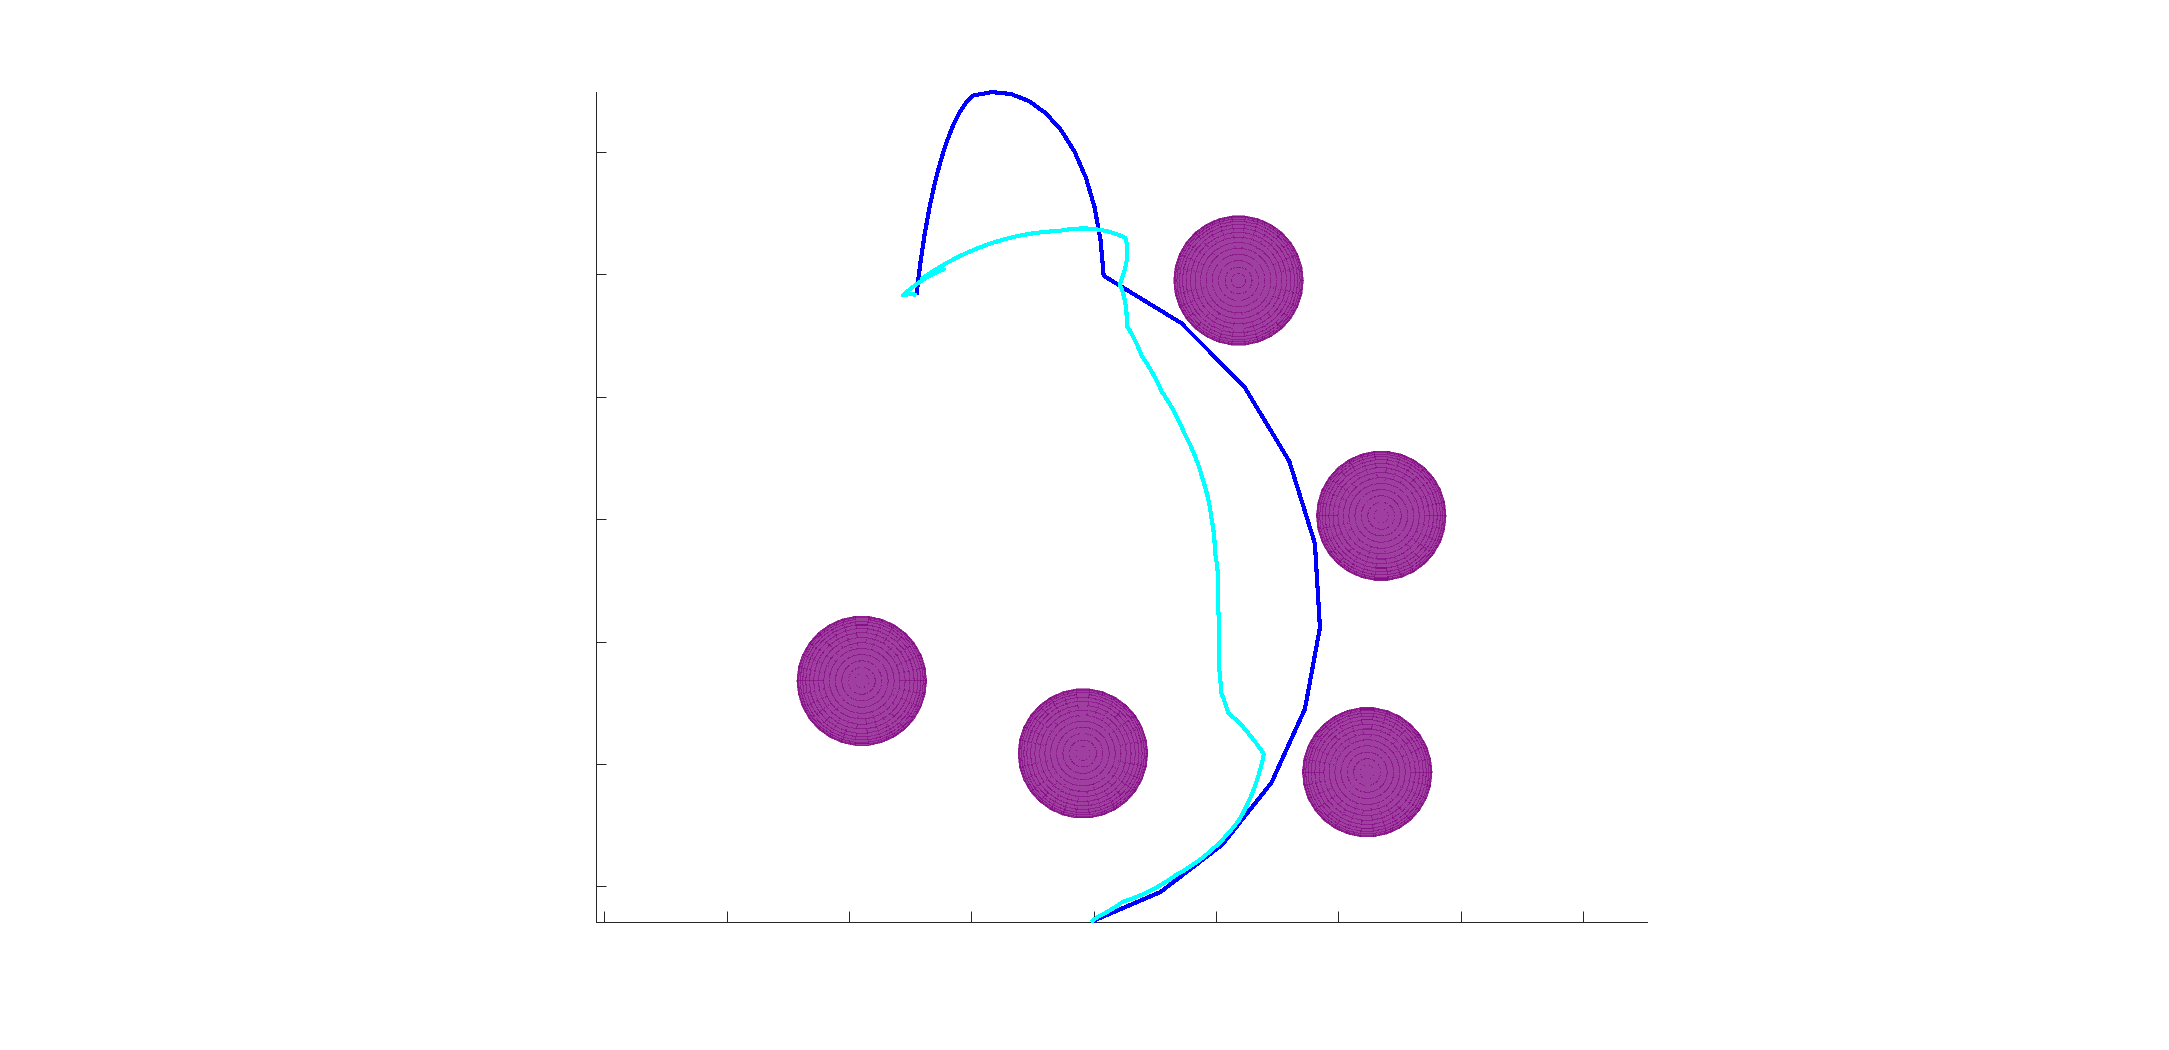
\includegraphics[width=0.2\textwidth]{Immagini/pdf/problem_B_01.eps}} \quad
%\subfloat[]{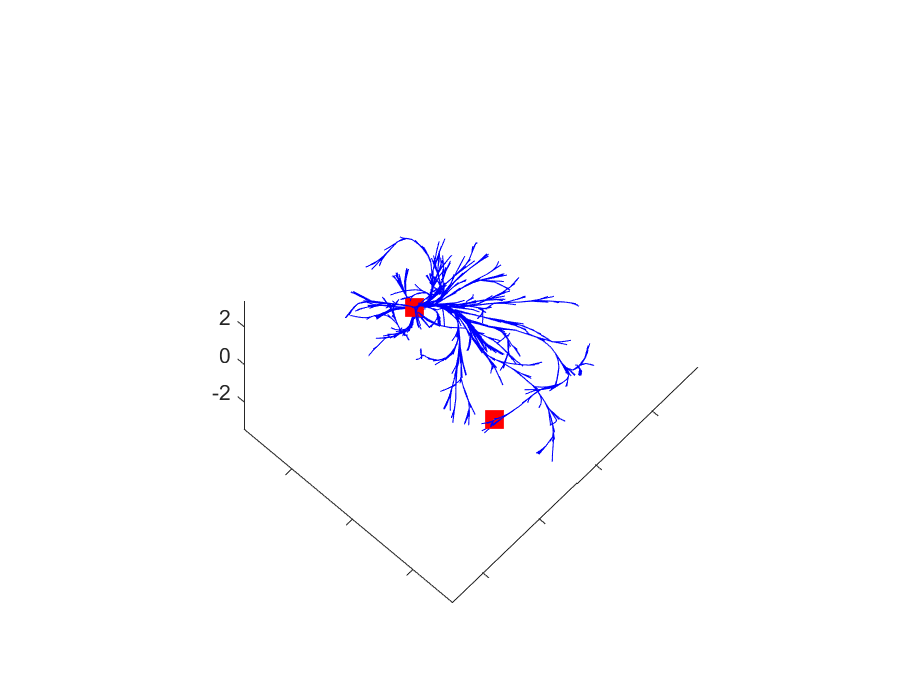
\includegraphics[width=0.2\textwidth]{Immagini/pdf/problem_B_02.eps}}
%\caption{On the left, the trajectory found by the RRT* algorithm as a solution to Problem B (cyan) in comparison to the solution found when considering a pure path planning problem (blue), i.e. problem A. On the right the tree obtained by the RRT* when solving problem B. METTERE spiegare perchè è diverso da path planning normale.}
%\end{figure}

\subsection{Results}

Figures \ref{fig:res_parall_query}, \ref{fig:res_shared}, \ref{fig:res_copied} and \ref{fig:res_ants} report the performance obtained when applying the strategies contained in MT-RRT, i.e. those described in Section \ref{sec:cap_03}, when varying the number of employed threads.
$\xi$ is the efficiency of the parallelization (normalized speed up, see \cite{efficiency_PC}), which is defined as follows (adopting the same notation of Section \ref{sec:cap_03}):
\begin{eqnarray}
\xi = \frac{T_{serial}}{T(P) \cdot P}
\end{eqnarray}
where $T_{serial}$ is the computation time absorbed by the standard serial versions presented in Section \ref{sec:cap_02}. In particular $T_{serial}$, was assumed as the mean value recorded for a batch of simulations. When having a good parallelization, $\xi$ should be close to 1 or higher. 
For all the simulations, the maximal number of iterations was set equal to 2500, and the termination criteria for all the versions adopting an RRT or a bidirectional RRT strategies was disabled: even in a case a solution was found, the search was not interrupted.
These results were obtained using a quad core laptop embedded with an Intel(R) core i7-6500u.

\begin{figure*}
	\centering
\subfloat[]{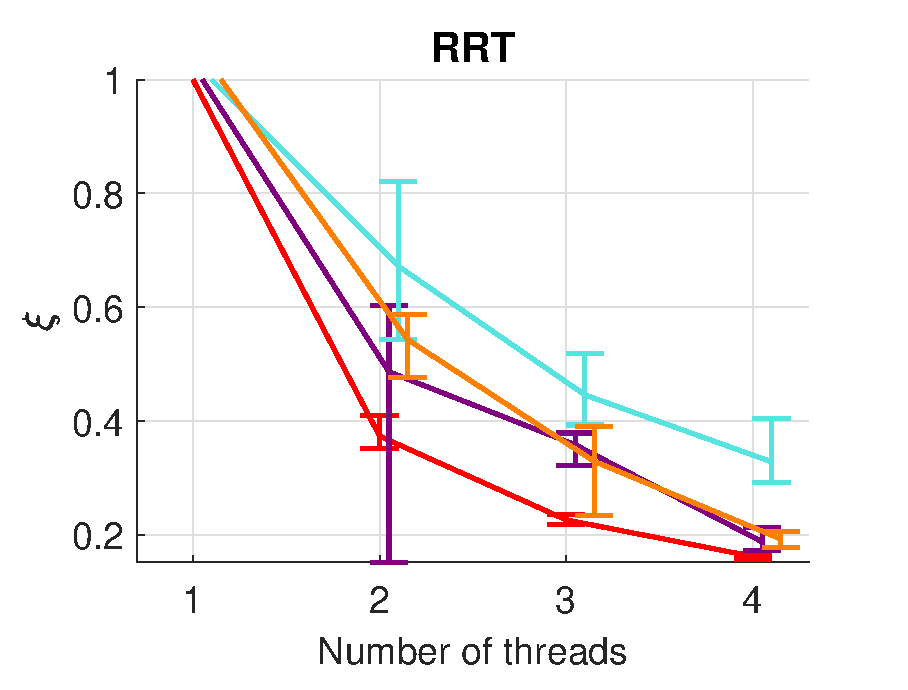
\includegraphics[width=0.31\textwidth]{Immagini/pdf/time_1_1.eps}} \quad
\subfloat[]{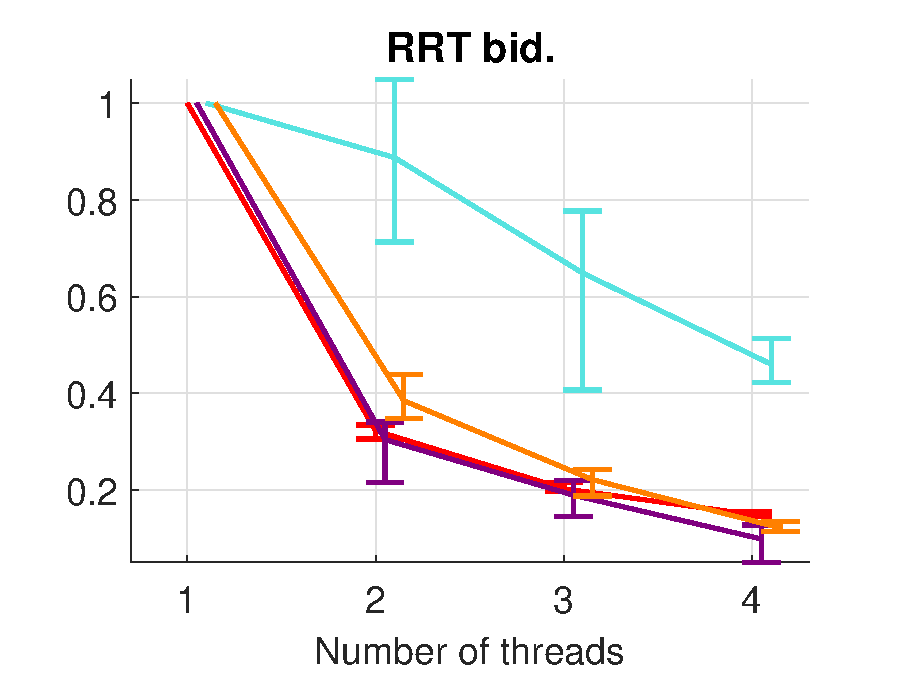
\includegraphics[width=0.31\textwidth]{Immagini/pdf/time_1_2.eps}} \quad
\subfloat[]{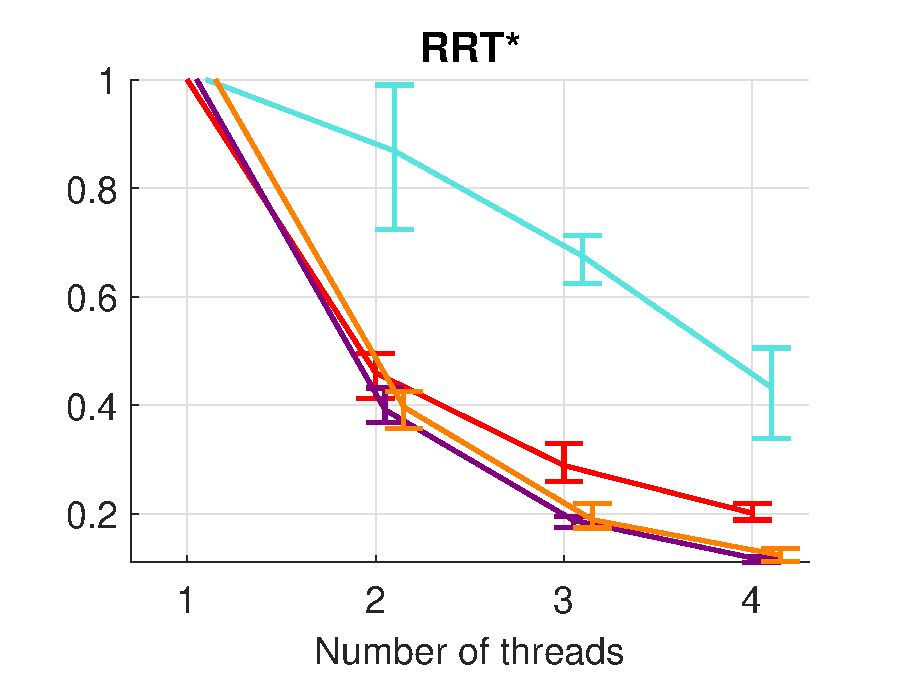
\includegraphics[width=0.31\textwidth]{Immagini/pdf/time_1_3.eps}} 
\caption{Performance obtained adopting the strategy described in Section \ref{subsec:MT_01}.}
\label{fig:res_parall_query}
\end{figure*}
\begin{figure*}
	\centering
\subfloat[]{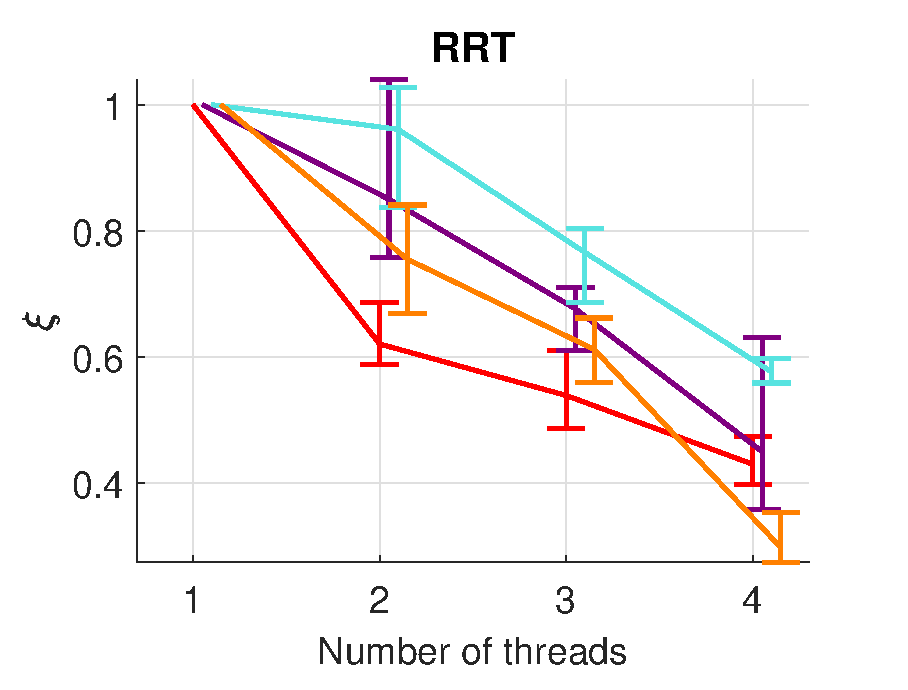
\includegraphics[width=0.31\textwidth]{Immagini/pdf/time_2_1.eps}} \quad
\subfloat[]{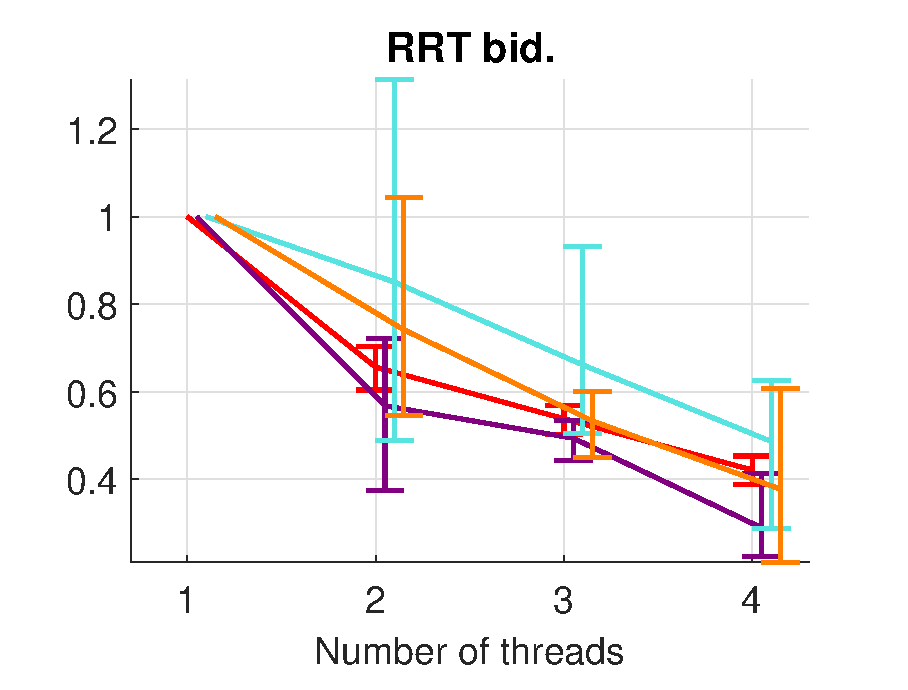
\includegraphics[width=0.31\textwidth]{Immagini/pdf/time_2_2.eps}} \quad
\subfloat[]{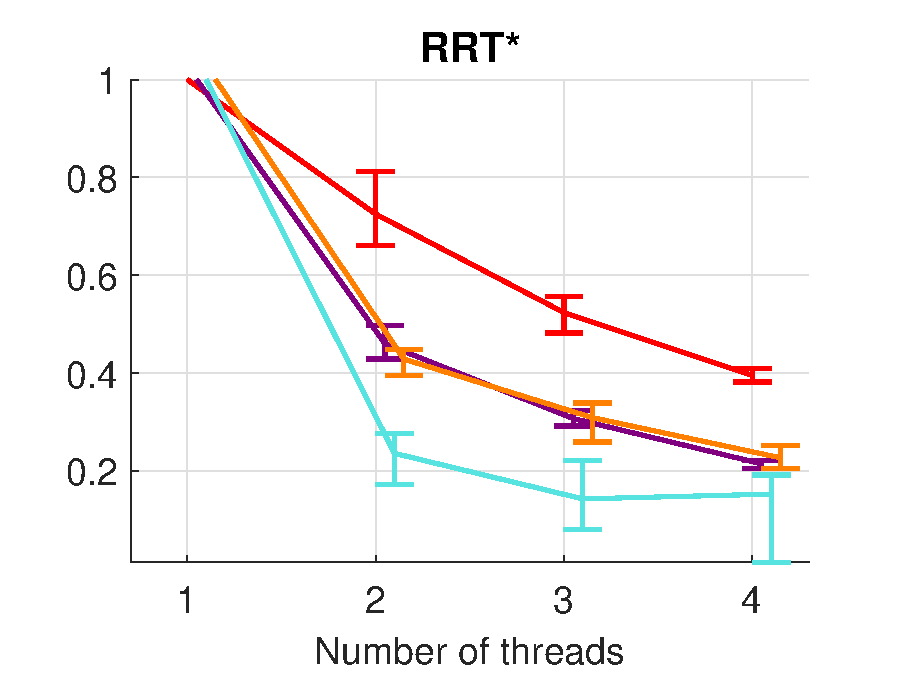
\includegraphics[width=0.31\textwidth]{Immagini/pdf/time_2_3.eps}} 
\caption{Performance obtained adopting the strategy described in Section \ref{subsec:MT_02}.}
\label{fig:res_shared}
\end{figure*}
\begin{figure*}
	\centering
\subfloat[]{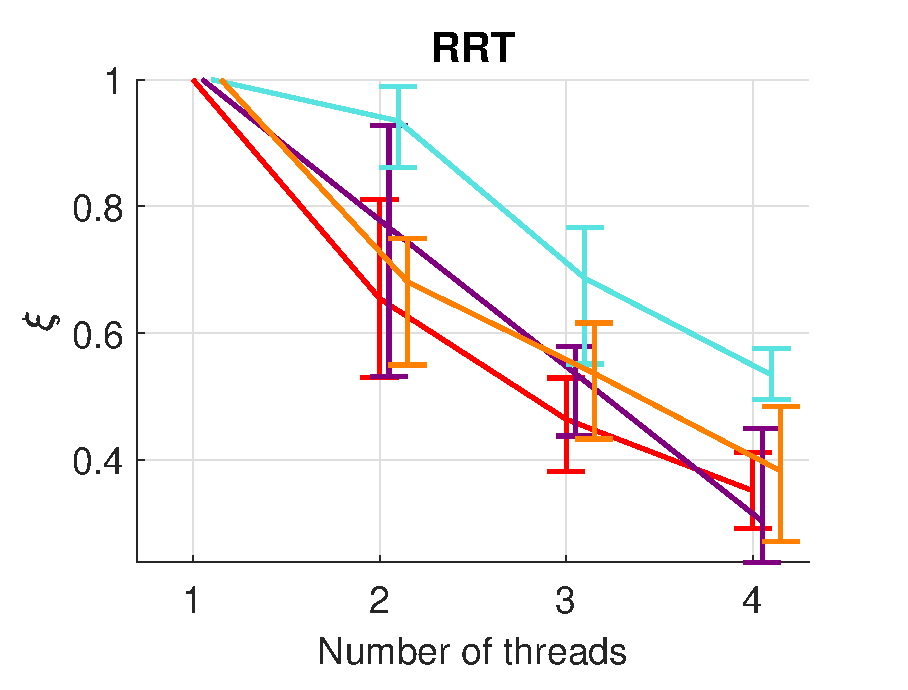
\includegraphics[width=0.31\textwidth]{Immagini/pdf/time_3_1.eps}} \quad
\subfloat[]{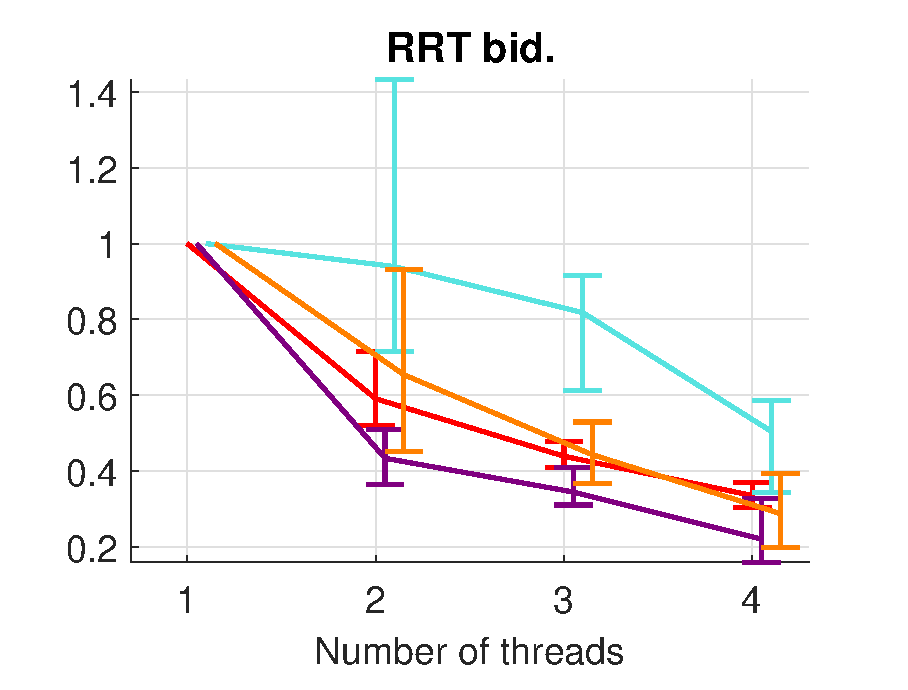
\includegraphics[width=0.31\textwidth]{Immagini/pdf/time_3_2.eps}} \quad
\subfloat[]{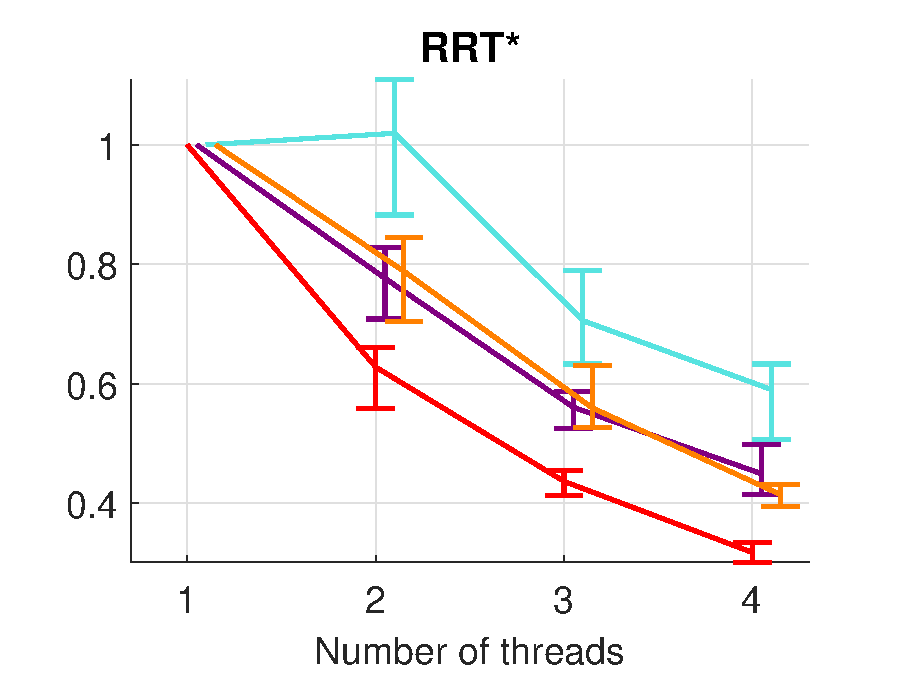
\includegraphics[width=0.31\textwidth]{Immagini/pdf/time_3_3.eps}} 
\caption{Performance obtained adopting the strategy described in Section \ref{subsec:MT_03}.}
\label{fig:res_copied}
\end{figure*}
\begin{figure*}
	\centering
\subfloat[]{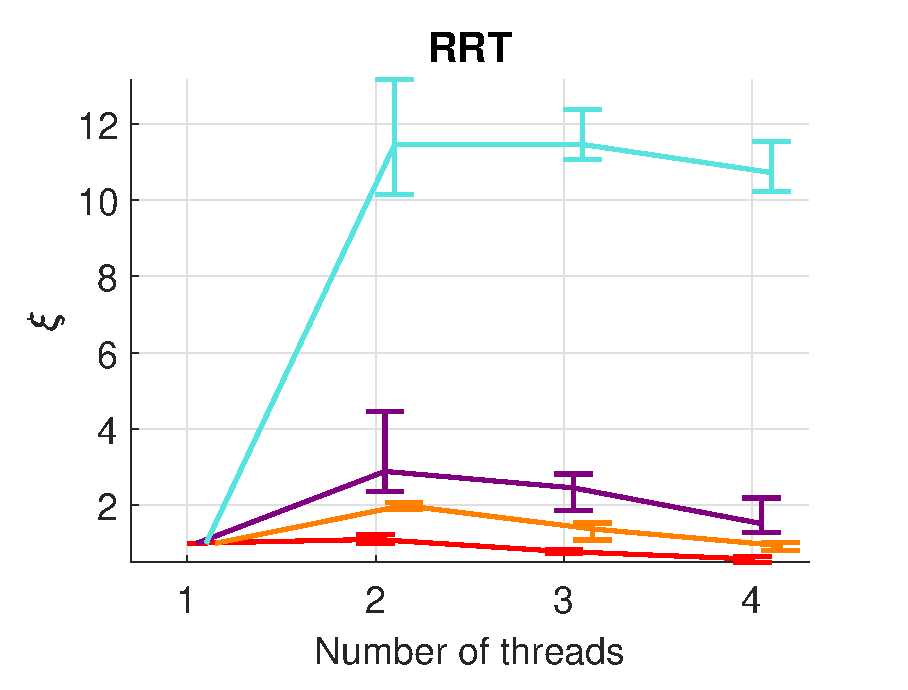
\includegraphics[width=0.31\textwidth]{Immagini/pdf/time_4_1.eps}} \quad
\subfloat[]{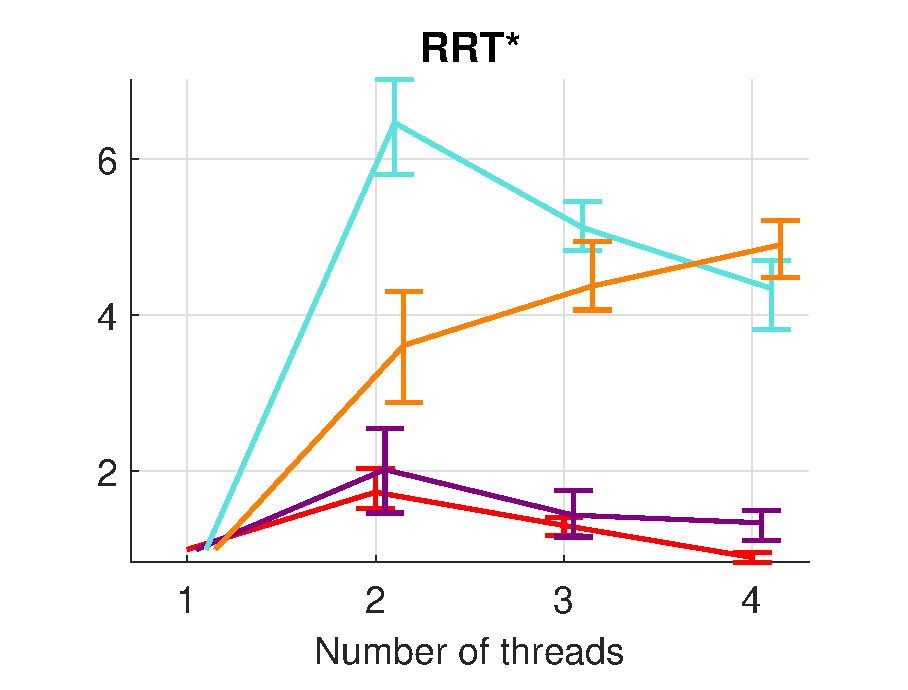
\includegraphics[width=0.31\textwidth]{Immagini/pdf/time_4_3.eps}} \quad
\subfloat[]{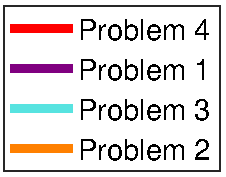
\includegraphics[width=0.15\textwidth]{Immagini/pdf/result_legenda.pdf}}
\caption{Performance obtained adopting the strategy described in Section \ref{subsec:MT_04}.}
\label{fig:res_ants}
\end{figure*}



\section{Conclusions}
\label{sec:conclusion}

The strategy presented in Section \ref{subsec:MT_01} results to be effective for Problem 3, i.e. the scenario for which $T_{\tau}  \gg T_V$, while for all the other problems its performance result to be poor in comparison to the other approaches. The reason is the presence of severe overhead times: after every collective search of the Nearest Neighbour or the determination of a Near set, threads must wait for all the others to end that search. Moreover, this happens at every iteration.
\\
The strategies reported in Sections \ref{subsec:MT_02} and \ref{subsec:MT_03} achieve comparable performance when considering the classical RRT and its bidirectional version, while for RRT* the approach presented in Section \ref{subsec:MT_03} outperforms the one of Section \ref{subsec:MT_02}. The reason is the presence of the critical sections for applying rewirds, which leads to time waste. 
\\
The multi agent approach of Section \ref{subsec:MT_04} is significantly faster w.r.t all the other methods for all the RRT versions considered, because threads perform parallel extensions on reduced-size trees. 
However, when considering the RRT* algorithm, the approach in \ref{subsec:MT_04} is an approximation of the canonical version, that might lead to solutions that are near-optimal. Therefore, for those cases for which the optimality is crucial, the approach of Section \ref{subsec:MT_03} can be efficiently deployed.
The entire MT-RRT library is available at \cite{github_link}, which contains also detailed directions to derive a customized planning problem to be solved with the usage of MT-RRT.
%\\
%It could be interesting for future studies to extend the proposed techniques for multi processing environments. Such approaches would achieve for sure slower computation times (because results must be communicate between threads because sharing memory it is not possible), but could be the only exploitable way for parallelizing an RRT problem when using different machines with their one processors and memory storage, with however a much bigger number of concurrent processes.



\bibliographystyle{IEEEtran}
\bibliography{IEEEabrv,bibliografia}

\end{document}
